\باب{توانائی اور برقی دباو}

\حصہ{توانائی اور کام}
قوت \عددیء{F} کی سمت میں فاصلہ \عددیء{\dif L} طے کرنے سے 
\begin{align*}
\dif W= F \dif L
\end{align*}
\اصطلاح{کام} کیا جاتا ہے۔اگر قوت اور طے کردہ فاصلہ ایک ہی سمت میں نہ ہوں تب  قوت کا وہ حصہ جو طے کردہ فاصلے کی سمت میں ہو اور طے شدہ فاصلے  کے حاصل ضرب کو \اصطلاح{کام}\فرہنگ{کام}\حاشیہب{work}\فرہنگ{work} کہتے ہیں۔شکل \حوالہ{شکل_دباو_کام_کی_تعریف} کو دیکھتے ہوئے سمتیات کے استعمال سے 
\begin{align*}
\dif W&=F \cos \alpha  \dif L\\
&=\kvec{F} \cdot \dif \kvec{L}
\end{align*}
لکھا جا سکتا ہے جہاں \عددیء{F \cos \alpha \dif L} کو نقطہ ضرب کی مدد سے \عددیء{\kvec{F} \cdot \dif \kvec{L}} لکھا گیا ہے۔
\begin{figure}
\centering
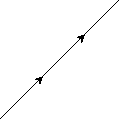
\includegraphics{figVoltageWork}
\caption{طے فاصلہ اور فاصلے کی سمت میں قوت کا حاصل ضرب کام کہلاتا ہے}
\label{شکل_دباو_کام_کی_تعریف}
\end{figure}

زمین اور کمیت \عددیء{m} کے درمیان قوت ثقل \عددیء{\kvec{F}_G=-\tfrac{GMm}{r^2}\ar} پایا جاتا ہے\حاشیہد{\عددیء{\ar}  اکائی سمتیہ ہے۔} جس میں \عددیء{\tfrac{GM}{r^2}=g} لکھتے ہوئے  \عددیء{\kvec{F}_G=-mg \ar} لکھا جا سکتا ہے۔کام کرتے ہوئے کمیت کو \عددیء{\Delta h \ar} اونچائی پر منتقل کرنے  کی خاطر قوت ثقل کے خلاف
\begin{align*}
\kvec{F}_{\textrm{لاگو}}=-\kvec{F}_G
\end{align*}
لاگو کرتے ہوئے
\begin{align*}
\Delta W=\kvec{F}_{\textrm{لاگو}} \cdot \Delta h \ar=mg \Delta h
\end{align*}
 توانائی درکار ہو گی۔کام کرنے کے لئے درکار توانائی کمیت میں منتقل ہو جاتی ہے جسے \اصطلاح{مخفی توانائی}\فرہنگ{مخفی توانائی}\حاشیہب{potential energy}\فرہنگ{potential energy} کہتے ہیں۔اگر \عددیء{\Delta h} کی قیمت  \عددیء{r} کی نسبت سے  بہت کم نہ ہو تب \عددیء{g} کو مستقل تصور کرنا ممکن نہ ہو گا اور مخفی توانائی تکملہ کے ذریعہ حاصل کی جائے گی۔
\begin{align*}
W =-\int_{\textrm{ابتدا}}^{\textrm{اختتام}} \kvec{F}_G \cdot \dif \kvec{r}=\int_{\textrm{ابتدا}}^{\textrm{اختتام}} \frac{GMm }{r^2} dr
\end{align*}
ثقلی میدان میں کمیت کو ابتدائی نقطے سے اختتامی نقطے تک پہنچاتے ہوئے کوئی بھی راستہ اختیار کیا جا سکتا ہے۔اختیار کردہ راستے کا مخفی توانائی پر کسی قسم کا کوئی اثر نہیں ہوتا۔ایسے میدان جن میں دو نقطوں کے مابین مخفففی توانائی کا دارومدار، ابتدائی نقطے سے اختتامی نقطے تک پہنچنے کے راستے،  پر نہیں ہوتا \اصطلاح{قائم میدان}\فرہنگ{قائم میدان}\حاشیہب{conservative field}\فرہنگ{conservative field} کہلاتے ہیں۔ 

برقی میدان میں چارجوں کے حرکت کے مسئلے کو بھی اسی طرح حل کیا جاتا ہے۔برقی میدان \سمتیہ{E} میں چارج \عددیء{q} پر قوت \عددیء{\kvec{F}_E=q \kvec{E}} عمل کرتا ہے۔چارج کو فاصلہ \عددیء{\dif \kvec{L}} ہلانے کی خاطر اس قوت کے خلاف بیرونی
\begin{align*}
\kvec{F}_{\textrm{لاگو}} = -\kvec{F}_E
\end{align*}
قوت لاگو کرتے ہوئے
\begin{align}\label{مساوات_دباو_کام_کی_تعریف}
\dif W=-q \kvec{E} \cdot \dif \kvec{L}
\end{align}
کام\حاشیہب{work} کیا جاتا ہے۔کسی بھی ابتدائی نقطے سے اختتامی نقطے تک یوں
\begin{align}\label{مساوات_دباو_لکیری_تکملہ}
W=-q \int_{\textrm{ابتدا}}^{\textrm{اختتام}} \kvec{E} \cdot \dif\kvec{L}
\end{align}
توانائی درکار ہو گی۔

\حصہ{لکیری تکملہ}\حاشیہط{مکمل کرنا درکار ہے۔}
مساوات \حوالہ{مساوات_دباو_لکیری_تکملہ} لکیری تکملہ ہے جس پر مزید غور کرتے ہیں۔شکل \حوالہ{شکل_دباو_تکملہ_بمع_مجموعہ} میں \اصطلاح{یکساں}\فرہنگ{یکساں}\حاشیہب{uniform}\فرہنگ{uniform} اور وقت کے ساتھ نہ تبدیل ہونے والے میدان  \عددیء{\kvec{E}} میں  نقطہ \عددیء{O} سے نقطہ \عددیء{N} تک  چارج  کی منتقلی دکھائی گئی ہے۔یکساں میدان سے مراد ایسا میدان ہے جس میں \عددیء{\kvec{E}}  کی قیمت جگہ جگہ تبدیل نہیں ہوتی بلکہ اس کی قیمت ہر جگہ یکساں ہوتی ہے۔اسی طرح وقت کے ساتھ تبدیل ہوتے میدان کو  وقت کے ساتھ تغیر پذیر میدان کہا جائے گا۔یکساں میدان وقت کے ساتھ غیر تغیر پذیر میدان ہے۔

\begin{figure}
\centering
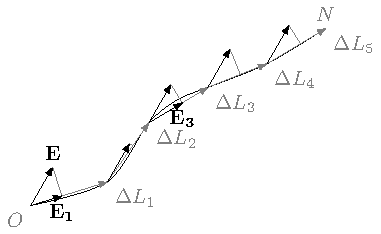
\includegraphics{figVoltageLineIntegralAsSum}
\caption{تکملہ دراصل چھوٹے حصوں کا مجموعہ ہوتا ہے۔}
\label{شکل_دباو_تکملہ_بمع_مجموعہ}
\end{figure}
شکل \حوالہ{شکل_دباو_تکملہ_بمع_مجموعہ} میں پورے راستے کو چھوٹے چھوٹے  ٹکڑے \عددیء{\Delta \kvec{L}_1}، \عددیء{\Delta \kvec{L}_2}، \عددیء{\cdots} میں تقسیم  کرتے ہوئے ایک ایک ٹکڑے پر حرکت کے لئے درکار توانائی مساوات \حوالہ{مساوات_دباو_کام_کی_تعریف} کی مدد سے  حاصل کی جا سکتی ہے۔یوں  \عددیء{\Delta \kvec{L}_1}  کے ابتدائی نقطے سے اختتامی نقطے تک چارج \عددیء{q} منتقل کرنے کی
 خاطر \عددیء{\Delta W=-q \kvec{E} \cdot \Delta \kvec{L}_1} توانائی درکار ہو گی۔یہی عمل راستے کے بقایا ٹکڑوں پر بھی لاگو کرتے ہوئے کُل درکار توانائی
\begin{gather}
\begin{aligned}\label{مساوات_دباو_مجموعہ_ٹکڑے}
W&=-q \kvec{E} \cdot \Delta \kvec{L}_1 -q \kvec{E} \cdot \Delta \kvec{L}_2 -q \kvec{E} \cdot \Delta \kvec{L}_3 -q \kvec{E} \cdot \Delta \kvec{L}_4 -q \kvec{E} \cdot \Delta \kvec{L}_5\\
&=-q \kvec{E} \cdot \left(\Delta \kvec{L}_1  +\Delta \kvec{L}_2 +\Delta \kvec{L}_3+\Delta \kvec{L}_4+\Delta \kvec{L}_5\right)
\end{aligned}
\end{gather}
لکھی جا سکتی ہے۔قوسین میں بند \عددیء{\Delta \kvec{L}_1  +\Delta \kvec{L}_2 +\Delta \kvec{L}_3+\Delta \kvec{L}_4+\Delta \kvec{L}_5} درحقیقت نقطہ \عددیء{O} سے \عددیء{N} تک کا  کُل سمتی راستہ \عددیء{\kvec{L}_{ON}} ہے۔یوں مندرجہ بالا مساوات کو
\begin{align}
W=-q \kvec{E} \cdot \kvec{L}_{ON}
\end{align}
لکھا جا سکتا ہے۔اگر شکل \حوالہ{شکل_دباو_تکملہ_بمع_مجموعہ} میں منتقلی کے راستے کے نہایت چھوٹے چھوٹے ٹکڑے \عددیء{\dif \kvec{L}} بنائے جائیں تو مساوات \حوالہ{مساوات_دباو_مجموعہ_ٹکڑے} کو تکمل کی شکل میں یوں لکھا جا سکتا ہے۔
\begin{align}
W=\int_O^N -q \kvec{E} \cdot \dif \kvec{L}
\end{align}
چونکہ \عددیء{q} اور \عددیء{\kvec{E}} کی قیمتیں مستقل ہیں  لہٰذا انہیں تکمل کے باہر لکھا جا سکتا ہے۔ایسا کرتے ہوئے
\begin{gather}
\begin{aligned}\label{مساوات_توانائی_یکساں_میدان_توانائی_راستے_پر_منحصر_نہیں}
W&=-q \kvec{E} \cdot  \int_O^N \dif \kvec{L}\\
&=-q \kvec{E} \cdot \kvec{L}_{ON}
\end{aligned}
\end{gather}
حاصل ہوتا ہے۔اس جواب سے ہم دیکھتے ہیں کہ درکار توانائی کا دارومدار \عددیء{q}، \عددیء{\kvec{E}} اور \عددیء{\kvec{L}_{ON}} پر ہے جہاں \عددیء{\kvec{L}_{ON}} نقطہ \عددیء{O} سے نقطہ \عددیء{N} تک سیدھی کھینچی لکیر ہے۔درکار توانائی کا اس سے کسی قسم کا کوئی تعلق نہیں کہ ابتدائی نقطے سے اختتامی نقطے جاتے ہوئے کون سا راستہ اختیار کیا گیا۔جیسا کہ پہلے ذکر کیا گیا، ایسے میدان کو \اصطلاح{قدامت پسند} میدان کہتے ہیں۔ہم جلد دیکھیں گے کہ غیر یکساں برقی میدان بھی قدامت پسند میدان ہوتا ہے البتہ تغیر پذیر  برقی میدان غیر قدامت پسند ہو سکتا ہے۔

\ابتدا{مثال}\شناخت{مثال_توانائی_سیدھی_لکیر_غیر_ہموار_میدان}
غیر یکساں، غیر تغیر پذیر میدان
\begin{align*}
\kvec{E}=(y+z)\ax+(x+z)\ay+(x+y)\az \quad \si{\volt \per \meter}
\end{align*}
میں \عددیء{N_1(1,0,2)} سے \عددیء{N_2(0,1,2)} تک سیدھی لکیر پر \عددیء{\SI{0.1}{\coulomb}} کا چارج منتقل کرنے کے لئے درکار توانائی حاصل  کریں۔ 
\begin{figure}
\centering
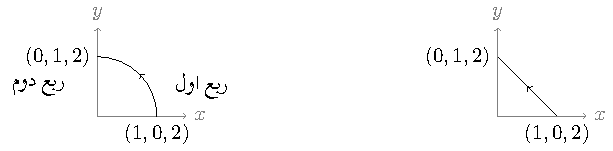
\includegraphics{figVoltageNonUniformNonTimeVaryingStraightLine}
\caption{چارج منتقل کرنے کے دو راستے۔}
\label{شکل_توانائی_چارج_منتقل_سیدھی_لکیر_گول_دائرہ}
\end{figure}

حل: شکل \حوالہ{شکل_توانائی_چارج_منتقل_سیدھی_لکیر_گول_دائرہ} میں چارج منتقل کرنے کا سیدھا راستہ دکھایا گیا ہے۔پہلے اس سیدھی لکیر کا مساوات حاصل کرتے ہیں۔اس لکیر کا ڈھلوان\حاشیہب{slope}
\begin{align*}
\textup{ڈھلوان}=m=\frac{y_2-y_1}{x_2-x_1}=\frac{1-0}{0-1}=-1
\end{align*}
 ہے لہٰذا سیدھی لکیر کی مساوات \عددیء{y=mx +c} میں نقطہ \عددیء{N_1} پُر کرتے ہوئے  \عددیء{0=-1 \times 1 +c} سے \عددیء{c=1} حاصل ہوتا ہے۔یوں لکیر کی مساوات
\begin{align}\label{مساوات_توانائی_سیدھی_لکیر_کی_مثال}
y=-x+1
\end{align}
ہے۔کارتیسی محدد میں کسی بھی راستے پر حرکت کرتے ہوئے  مساوات \حوالہ{مساوات_سمتیہ_کارتیسی_چھوٹا_فاصلہ} کے مطابق
\begin{align}
\dif \kvec{L}=\dif x \ax+\dif y \ay+\dif z \az
\end{align}
لکھا جاتا ہے۔یوں مساوات \حوالہ{مساوات_دباو_لکیری_تکملہ} سے حاصل ہو گا۔
\begin{align*}
W&=-q \int_{\textrm{ابتدا}}^{\textrm{اختتام}} \kvec{E} \cdot \dif\kvec{L}\\
&=-0.1 \int_{N_1}^{N_2} \left[ (y+z)\ax+(x+z)\ay+(x+y)\az \right] \cdot (\dif x \ax+\dif y \ay+\dif z \az)\\
&=-0.1 \int_{1}^{0} (y+z) \dif x -0.1 \int_{0}^{1}(x+z) \dif y-0.1 \int_{2}^{2} (x+y) \dif z
\end{align*}
آخری قدم پر تکمل کو تین حصوں میں لکھا گیا ہے جہاں پہلے حصے میں تکمل کو \عددیء{x} کے ساتھ حاصل کیا گیا ہے جبکہ دوسرے حصے میں تکمل کو \عددیء{y} کے ساتھ اور آخری حصے میں اسے \عددیء{z} کے ساتھ حاصل کیا گیا ہے۔پہلے حصے میں \عددیء{(y+z)} کا تکمل \عددیء{x} کے ساتھ ہے لہٰذا  \عددیء{(y+z)} کو \عددیء{x} کی صورت میں لکھنا ہو گا۔منتقلی کے راستے  پر \عددیء{z=2} ہے جبکہ  مساوات \حوالہ{مساوات_توانائی_سیدھی_لکیر_کی_مثال} میں \عددیء{y} کو \عددیء{x} کی صورت میں لکھا گیا ہے۔یوں پہلا تکمل
\begin{align*}
-0.1 \int_{1}^{0} [y+z]\dif x &=-0.1 \int_{1}^{0} [(-x+1)+2] \dif x\\
&=-0.1\left.\left(\frac{-x^2}{2}+3x\right) \right|_{1}^{0}\\
&=\SI{0.25}{\joule}
\end{align*}
یعنی جاول کے ایک چوتھائی کے برابر حاصل ہوتا ہے۔دوسرا تکمل \عددیء{y} کے ساتھ ہے لہٰذا تمام متغیرات  \عددیء{y} کی صورت میں لکھنے ہوں گے۔سیدھی لکیر کے مساوات سے  \عددی{x=-y+1} لکھا جا سکتا ہے جبکہ  پورے راستے پر \عددیء{z=2}  کے برابر ہے لہٰذا
\begin{align*}
-0.1 \int_{0}^{1} [x+z]\dif y &=-0.1 \int_{0}^{1} [(-y+1)+2] \dif y\\
&=-0.1 \left.\left(\frac{-y^2}{2}+3y\right) \right|_{0}^{1}\\
&=\SI{-0.25}{\joule}
\end{align*}
ہو گا۔تیسرے تکمل میں ابتدائی اور اختتامی نقطے ایک ہی ہیں لہٰذا یہ تکمل صفر کے برابر ہے۔ 
\begin{align*}
-0.1 \int_{2}^{2} (x+y) \dif z &=\SI{0}{\joule}
\end{align*}
اس طرح کُل درکار توانائی تینوں جوابات کا مجموعہ یعنی  \عددیء{\SI{0}{\joule}} ہو گی۔مثبت جواب کا مطلب یہ ہے کہ چارج کو منتقل کرنے کی خاطر بیرونی لاگو قوت توانائی فراہم کرے گی۔ 
\انتہا{مثال}
%=============
\ابتدا{مثال}
گزشتہ مثال میں سیدھی لکیر پر چارج منتقل کرنے کے لئے درکار توانائی حاصل کرنے کو کہا گیا۔اس مثال میں شکل \حوالہ{شکل_توانائی_چارج_منتقل_سیدھی_لکیر_گول_دائرہ} میں بائیں جانب گول دائرے کے راستے \عددیء{(1,0,2)} سے \عددیء{(0,1,2)} تک \عددیء{\kvec{E}=(y+z)\ax+(x+z)\ay+(x+y)\az \, \si{\volt \per \meter}} میدان میں \عددیء{\SI{0.1}{\coulomb}} کے چارج کو منتقل کرنے کی خاطر درکار توانائی حاصل کریں۔گول دائرے کا راستہ \عددیء{z=2} سطح پر پایا جاتا ہے۔

حل:اکائی رداس کے گول دائرے کی مساوات \عددیء{x^2+y^2=1^2} ہے۔یوں مساوات \حوالہ{مساوات_دباو_لکیری_تکملہ} سے حاصل تین تکملوں
\begin{align*}
W&=-0.1 \int_{1}^{0} (y+z) \dif x -0.1 \int_{0}^{1}(x+z) \dif y-0.1 \int_{2}^{2} (x+y) \dif z
\end{align*}
میں پہلی تکمل میں \عددیء{z=2} اور \عددیء{y=\sqrt{1-x^2}} پُر کرنا ہو گا۔یاد رہے کہ ربع اول\فرہنگ{ربع اول}\حاشیہب{first quadrant}\فرہنگ{quadrant} میں \عددیء{x} اور \عددیء{y} دونوں کی قیمتیں مثبت ہوتی ہیں۔اس طرح کے تکمل حل کرتے وقت ربع کو مد نظر رکھنا ضروری ہے۔ 
\begin{align*}
-0.1 \int_{1}^{0} (y+z) \dif x&=-0.1\int_{1}^{0} (\sqrt{1-x^2}+2) \dif x\\
&=-0.1\left.(\frac{\sin^{-1} x}{2}+\frac{x \sqrt{1-x^2}}{2}+2x)\right|_1^0\\
&=-0.025 \pi-0.2
\end{align*}
جاول، دوسرے تکمل میں \عددیء{z=2} ہی رہے گا جبکہ \عددیء{x=\mp \sqrt{1-y^2}} میں سے \عددیء{x=\sqrt{1-y^2}} کا استعمال ہو گا۔یوں
\begin{align*}
-0.1 \int_{0}^{1}(x+z) \dif y&=-0.1\int_{0}^{1} (\sqrt{1-y^2}+2) \dif y\\
&=-0.1\left.(\frac{\sin^{-1} y}{2}+\frac{y \sqrt{1-y^2}}{2}+2x)\right|_0^1\\
&=0.025 \pi+0.2
\end{align*}
جاول حاصل ہوتا ہے۔ تیسرے تکمل میں ابتدائی اور اختتامی نقطے ایک ہی ہیں لہٰذا یہ تکمل صفر کے برابر ہے۔ 
\begin{align*}
-0.1 \int_{2}^{2} (x+y)  \dif z =\SI{0}{\joule}
\end{align*}
کُل توانائی ان تین جوابات کا مجموعہ یعنی \عددیء{\SI{0}{\joule}} ہو گا۔
\انتہا{مثال}
%===========
\ابتدا{مشق}
گزشتہ دو مثالوں میں ابتدائی نقطہ \عددیء{(1,0,2)} اور اختتامی نقطہ \عددیء{(\tfrac{1}{\sqrt{2}},\tfrac{1}{\sqrt{2}},2)} تصور کرتے ہوئے دوبارہ حل کریں۔

جوابات:  $\SI{-0.1328}{\joule}$، $\SI{-0.1328}{\joule}$
\انتہا{مشق}


محدد کے مرکز پر موجود نقطہ چارج \عددیء{Q} کا میدان ہم حاصل کر چکے ہیں جسے یہاں دوبارہ پیش کرتے ہیں۔
\begin{align}
\kvec{E}=\frac{Q}{4 \pi \epsilon_0 r^2} \ar
\end{align}
آئیں دیکھیں کہ رداس تبدیل کئے بغیر اس میدان میں چارج \عددیء{q} کو حرکت دیتے ہوئے کتنی توانائی درکار ہو گی۔چونکہ میدان رداس کی سمت میں ہے اور رداس تبدیل کئے بغیر حرکت صرف اُس صورت ممکن ہے کہ ہم \عددیء{\ar} یعنی \عددیء{\kvec{E}} کے عمود میں سفر کریں۔ایسی صورت میں چارج پر میدان سے رونما ہونے والی قوت اور طے فاصلہ عمودی ہوں گے لہٰذا درکار توانائی صفر کے برابر ہو گی۔آئیں تکمل کے ذریعہ یہی جواب حاصل کریں۔
\begin{figure}
\centering
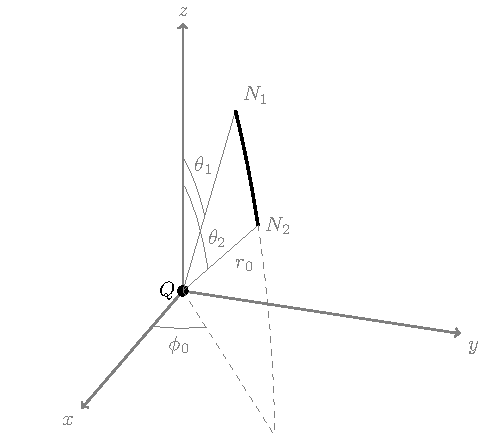
\includegraphics{figEnergyLineIntegralAlongTheta}
\caption{نقطہ چارج کے گرد صرف \عددیء{\theta} تبدیل کرتے ہوئے حرکت کا راستہ}
\label{شکل_توانائی_نقطہ_چارج_کے_گرد_تھیٹا_تبدیل_کرتے_راستہ}
\end{figure}

تصور کریں کہ \عددیء{\phi=\phi_0} اور \عددیء{r=r_0} رکھتے ہوئے ہم \عددیء{\theta} کو \عددیء{\theta_1} تا \عددیء{\theta_2} ریڈیئن  تبدیل کرتے ہوئے  چارج کو نقطہ \عددیء{N_1} سے  \عددیء{N_2} تک حرکت دیتے ہیں۔یہ صورت حال شکل \حوالہ{شکل_توانائی_نقطہ_چارج_کے_گرد_تھیٹا_تبدیل_کرتے_راستہ} میں دکھائی گئی ہے۔مساوات \حوالہ{مساوات_سمتیہ_کارتیسی_چھوٹا_فاصلہ}، مساوات \حوالہ{مساوات_سمتیہ_نلکی_چھوٹا_فاصلہ} اور مساوات \حوالہ{مساوات_سمتیہ_کروی_چھوٹا_فاصلہ} جنہیں یہاں دوبارہ پیش کرتے ہیں
\begin{gather}
\begin{aligned}
\dif \kvec{L}&=\dif x \ax+\dif y \ay+\dif z \az \\
\dif \kvec{L}&=\dif \rho \arho+\rho \dif \phi \aphi+\dif z \az\\
\dif \kvec{L}&=\dif r \ar+ r \dif \theta \atheta+r \sin \theta \dif \phi \aphi
\end{aligned}
\end{gather} 
کارتیسی، نلکی اور کروی متغیرات تبدیل کرنے سے پیدا چھوٹا فاصلہ \عددیء{\dif \kvec{L}} دیتے ہیں۔یوں درکار توانائی
\begin{align*}
W&=-q\int_{\textup{ابتدا}}^{\textup{اختتام}} \kvec{E} \cdot \dif \kvec{L}\\
&=-q \int_{r_0, \theta_1,\phi_0}^{r_0,\theta_2,\phi_0}\frac{Q}{4 \pi \epsilon_0 r^2} \ar \cdot (\dif r \ar+ r \dif \theta \atheta+r \sin \theta \dif \phi \aphi)\\
&=-q \int_{r_0}^{r_0}\frac{ Q \dif r}{4 \pi \epsilon_0 r^2}\\
&=0
\end{align*}
صفر ہی حاصل ہوتی ہے۔یہاں دوسرے قدم پر \عددیء{\ar \cdot \ar=1} کے علاوہ \عددیء{\ar \cdot \atheta=0} اور \عددیء{\ar \cdot \aphi=0} کا استعمال کیا گیا۔

اس کے برعکس اگر نقطہ \عددیء{(r_1,\theta_1,\phi_1)} تا نقطہ \عددیء{(r_2,\theta_2,\phi_2)} چارج کو حرکت دی جائے تب
\begin{align*}
W&=-q \int_{r_1, \theta_1,\phi_1}^{r_2,\theta_2,\phi_2}\frac{Q}{4 \pi \epsilon_0 r^2} \ar \cdot (\dif r \ar+ r \dif \theta \atheta+r \sin \theta \dif \phi \aphi)\\
&=-q \int_{r_1}^{r_2}\frac{ Q \dif r}{4 \pi \epsilon_0 r^2}\\
&=\frac{qQ}{4 \pi \epsilon_0} \left(\frac{1}{r_2}-\frac{1}{r_1} \right)
\end{align*}
ہو گا۔ یوں \عددیء{r_1 > r_2} کی صورت میں جواب مثبت ہو گا اور چارج کو ابتدائی نقطے سے اختتامی نقطے منتقل کرنے کے خاطر بیرونی توانائی درکار ہو گی جبکہ \عددیء{r_2>r_1} کی صورت میں جواب منفی حاصل ہوتا ہے لہٰذا چارج کے حرکت سے ہمیں توانائی حاصل ہو گی۔
%=====
\ابتدا{مشق}
میدان \عددیء{\kvec{E}=3x^2yz^2 \ax+x^3z^2\ay+2x^3yz\az \, \si{\volt \per \meter}} میں محدد کے مرکز \عددیء{(0,0,0)} سے نقطہ \عددیء{(2,3,5)} تک دو کولمب کا چارج مندرجہ ذیل راستوں منتقل کرنے کے لئے درکار توانائی حاصل کریں۔

\begin{itemize}
\item
دو نقطوں کے مابین سیدھی لکیر۔
\item
ایسا راستہ جس پر \عددیء{y=\tfrac{3}{4}x^2} اور \عددیء{z=\frac{x}{2}+x^2} ہوں۔
\end{itemize}

جوابات: سیدھی لکیر پر \عددیء{y=\tfrac{3}{2}x} اور \عددیء{z=\tfrac{5}{2}x} لکھا جائے گا۔جوابات کے مطابق توانائی درکار نہیں بلکہ حاصل ہو گی۔\عددیء{\SI{-1200}{\joule}}، \عددیء{\SI{-1200}{\joule}} 
\انتہا{مشق}
%============
\حصہ{برقی دباو}
چارج \عددیء{q} کے منتقلی کے لئے درکار  توانائی سے زیادہ اہم  اکائی چارج کے منتقلی کے لئے درکار توانائی ہے۔اس توانائی کو \اصطلاح{برقی دباو}\فرہنگ{برقی دباو}\حاشیہب{voltage}\فرہنگ{voltage} کہتے  ہیں۔برقی دباو کے اکائی \عددیء{\si{\joule / \coulomb}} کو \اصطلاح{وولٹ}\فرہنگ{وولٹ}\حاشیہب{volt}\فرہنگ{volt} کا نام دیا گیا ہے جسے \عددیء{\si{\volt}} سے ظاہر کیا جاتا ہے۔چونکہ توانائی غیر سمتی یعنی مقداری ہے لہٰذا برقی دباو بھی مقداری ہے۔مساوات \حوالہ{مساوات_دباو_لکیری_تکملہ} سے برقی دباو یوں حاصل ہوتا ہے
\begin{align}\label{مساوات_توانائی_برقی_دباو_تعریف}
V_{AB}=\frac{W}{q}=-\int_{B}^{A} \kvec{E} \cdot \dif\kvec{L}
\end{align}
جہاں ابتدائی نقطے کو \عددیء{B}، اختتامی نقطے کو \عددیء{A} اور حاصل جواب کو \عددیء{V_{AB}} لکھا گیا ہے۔\عددیء{V_{AB}} لکھتے ہوئے زیر نوشت میں پہلے اختتامی نقطہ  \عددیء{A} اور بعد میں ابتدائی نقطہ \عددیء{B} لکھا گیا ہے۔مساوات \حوالہ{مساوات_توانائی_یکساں_میدان_توانائی_راستے_پر_منحصر_نہیں} میں فاصلہ \عددیء{\kvec{L}_{ON}} لکھتے ہوئے زیر نوشت میں ابتدائی نقطہ \عددیء{O} پہلے اور اختتامی نقطہ \عددیء{N} بعد میں لکھا گیا۔برقی دباو  \عددیء{V_{AB}} لکھتے ہوئے اس فرق کو مدنظر رکھنا ہو گا۔

برقی دباو دو نقطوں کے مابین ناپی جاتی ہے۔کسی نقطے کی حتمی برقی دباو معنی نہیں رکھتی۔برقی دباو بالکل اونچائی کے مترادف ہے۔یوں کسی پہاڑی کے قریب کھڑے ہو کر اگر اس کی اونچائی تین سو میٹر ناپی جائے تو اسی پہاڑی کی اونچائی سطح سمندر سے ناپتے ہوئے سات سو میٹر حاصل ہو سکتی ہے۔آپ دیکھ سکتے ہیں کہ اونچائی ناپتے ہوئے \اصطلاح{نقطہ حوالہ}\فرہنگ{حوالہ!نقطہ}\حاشیہب{reference point}\فرہنگ{reference point}، جہاں کی نسبت سے اونچائی ناپی جائے، نہایت اہمیت کا حامل  ہے۔\اصطلاح{نقطہ حوالہ} کی اونچائی صفر تصور کی جاتی ہے۔دو یا دو سے زیادہ  عمارتوں کی اونچائی کا موازنہ کرتے وقت ان تمام عمارتوں کی اونچائی پہلے کسی ایک نقطے سے ناپی جاتی ہے۔یہ نقطہ عموماً زمین کی سطح ہوتی ہے۔اس کے برعکس مختلف شہروں یا پہاڑیوں کی اونچائی عموماً سطح سمندر سے ناپی جاتی ہے۔اگر تمام افراد کسی ایک \اصطلاح{نقطہ حوالہ} پر اتفاق کریں تب اس نقطے کی نسبت سے کسی مقام کی اونچائی کو اس مقام کی حتمی اونچائی تصور کی جاتی ہے۔ بالکل اسی طرح مختلف نقطوں کے برقی دباو کا موازنہ کرتے ہوئے ان تمام نقطوں کی برقی دباو کسی ایک نقطے کی نسبت سے ناپے جائیں گے۔ایسے نقطے کو \اصطلاح{برقی زمین}\فرہنگ{برقی زمین}\حاشیہب{electrical ground}،\فرہنگ{ground} کہا جاتا ہے جہاں برقی زمین کو صفر  برقی دباو پر تصور کیا جاتا ہے۔عموماً کرہ ارض کی سطح کو ہی برقی زمین تصور کیا جاتا ہے۔

موٹر گاڑی میں نسب بیٹری کے مثبت سرے کی برقی دباو،  بیٹری کے منفی سرے کی نسبت سے ناپنا زیادہ مطلب آمیز ہو گا جبکہ گھریلو برقی دباو مہیا کردہ ٹھنڈی اور گرم تار کے مابین ناپنا مطلب رکھتا ہے۔کبھی کبھار برقی دباو ناپنا نسبتاً مشکل ہوتا ہے، مثلاً  کرہ ارض  کی برقی دباو کو کس نقطہ حوالہ سے ناپا جائے گا۔طبیعیات کے میدان میں عموماً ایسے ہی مسئلے درپیش آتے ہیں جہاں نقطہ حوالہ تعین کرنا دشوار ہوتا ہے۔ایسی صورت میں نقطہ حوالہ کو لامحدود فاصلے پر تصور کیا جاتا ہے اور نقطہ \عددیء{A} کے برقی دباؤ کو \عددیء{V_A} لکھا جاتا ہے۔یوں لامحدود فاصلے سے اکائی چارج کو کرہ ارض تک لانے کے لئے درکار توانائی دریافت کرتے ہوئے کرہ ارض کی برقی دباو حاصل کی جائے گی۔

ہمہ محوری تار کے مسائل پر غور کرتے ہوئے عموماً اس کی بیرونی نلکی سطح کو نقطہ حوالہ لیا جاتا ہے۔اسی طرح کروی تناسب رکھنے والے سطحوں کے مابین برقی دباو حاصل کرتے وقت ان میں کسی ایک سطح کو حوالہ سطح چنا جائے گا۔

اگر نقطہ \عددیء{A} کی برقی دباو \عددیء{V_A} جبکہ نقطہ \عددیء{B} کی برقی دباو \عددیء{V_B} ہو تب ان کے مابین برقی دباو 
\begin{align}
V_{AB}=V_A-V_B
\end{align}
ہو گا جہاں نقطہ \عددیء{B} کو نقطہ حوالہ تصور کیا گیا ہے۔یہ مساوات صرف اور صرف اسی صورت درست ہو گی جب \عددیء{V_A} اور  \عددیء{V_B} ازخود  ایک ہی نقطہ حوالہ سے ناپے گئے ہوں۔
%==============================

\جزوحصہ{نقطہ چارج کا برقی دباو}
شکل \حوالہ{شکل_توانائی_نقطہ_چارج_دباو}  میں خالی خلاء میں کروی محدد کے مرکز پر پائے جانے والے چارج \عددیء{Q} کے میدان میں کسی بھی راستے پر  \عددیء{q} کولمب  کے پیمائشی چارج کو نقطہ \عددیء{B} سے نقطہ \عددیء{A} لانا دکھایا گیا ہے۔\عددیء{Q} سے \عددیء{r} فاصلے پر اس راستے کے چھوٹی لمبائی \عددیء{\dif \kvec{L}} پر اوسط برقی میدان \عددیء{\kvec{E}=\tfrac{Q}{4\pi \epsilon_0 r^2}\ar} ہو گا۔یوں اتنا راستہ طے کرنے کے لئے
\begin{align*}
\dif W&=- q \kvec{E} \cdot \dif \kvec{L}\\
&=-q \left(\frac{Q}{4\pi \epsilon_0 r^2}\ar \right) \cdot \left(\dif r \ar+r \dif \theta \atheta+r \sin \theta \dif \phi \aphi \right)\\
&=-\frac{q Q \dif r}{4 \pi \epsilon_0 r^2}
\end{align*}
توانائی درکار ہو گی۔اس طرح پورا راستہ طے کرنے کے لئے
\begin{align*}
W=-\int_{r_B}^{r_A} \frac{qQ \dif r}{4 \pi \epsilon_0 r^2}=\left. \frac{qQ}{4\pi \epsilon_0 r}\right|_{r_B}^{r_A}=\frac{qQ}{4\pi \epsilon_0} \left( \frac{1}{r_A}-\frac{1}{r_B} \right)
\end{align*}
%
\begin{figure}
\centering
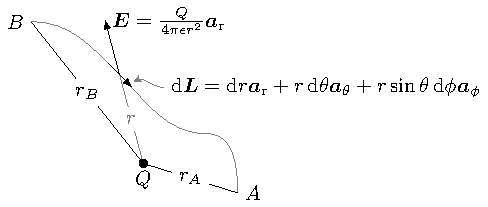
\includegraphics{figEnergyPotentialOfPointCharge}
\caption{نقطہ چارج کی برقی دباو۔}
\label{شکل_توانائی_نقطہ_چارج_دباو}
\end{figure}
توانائی درکار ہو گی جس سے ان دو نقطوں کے مابین برقی دباو \عددیء{V_{AB}=\tfrac{W}{q}} یوں حاصل ہوتا ہے۔
\begin{align}\label{مساوات_توانائی_نقطہ_چارج_کی_دباو}
V_{AB}=\frac{Q}{4\pi \epsilon_0} \left( \frac{1}{r_A}-\frac{1}{r_B} \right)
\end{align}

اس مساوات سے صاف ظاہر ہے کہ نقطہ چارج \عددیء{Q} کے میدان میں دو نقطوں کے مابین برقی دباو کا انحصار چارج سے نقطوں کے فاصلوں \عددیء{r_A} اور \عددیء{r_B} پر ہے نا کہ ایک نقطے سے دوسرے نقطے تک پہنچنے کے راستے پر۔یوں نقطہ \عددیء{B} کے حوالے سے نقطہ \عددیء{A} پر برقی دباو مساوات \حوالہ{مساوات_توانائی_نقطہ_چارج_کی_دباو} سے حاصل ہوتا ہے۔اگر نقطہ \عددیء{B} کو لامحدود فاصلے پر رکھا جائے یعنی اگر \عددیء{r_B =\infty} لیا جائے تب \عددیء{\tfrac{1}{\infty}=0} ہونے کی وجہ سے  یہ مساوات
\begin{align}\label{مساوات_توانائی_نقطہ_چارج_کی_حتمی_دباو}
V_{A}=\frac{Q}{4\pi \epsilon_0 r_A}
\end{align}
صورت اختیار کر لیتی ہے۔اگر ہم  حوالہ نقطہ کے لامحدود فاصلے پر ہونے پہ اتفاق کریں تو ایسی صورت میں \عددیء{\tfrac{Q}{4\pi\epsilon_0 r_A}} کو نقطہ \عددیء{A} کی حتمی برقی دباو تصور کیا جا سکتا ہے جسے \عددیء{V_A} لکھا جاتا ہے۔نقطہ حوالے کو لامحدود فاصلے پر رکھنے کا مطلب ہے کہ برقی زمین لامحدود فاصلے پر ہے۔ نقطہ حوالہ پر اتفاق کے بعد برقی دباو کی بات کرتے ہوئے بار بار برقی زمین کی نشاندہی کرنا ضروری نہیں لہٰذا برقی دباو لکھتے ہوئے زیر نوشت میں \عددیء{B} لکھنے سے گریز کیا جاتا ہے اور اسے صرف \عددیء{V_A} لکھا جاتا ہے۔مساوات \حوالہ{مساوات_توانائی_نقطہ_چارج_کی_حتمی_دباو} نقطہ \عددیء{A} کی حتمی برقی دباو دیتا ہے جو \عددیء{Q} سے \عددیء{r_A} فاصلے پر ہے۔یہ نقطہ کوئی بھی نقطہ ہو سکتا ہے لہٰذا  اسے  \عددیء{r_A} فاصلے پر نقطہ \عددیء{A} کی بجائے \عددیء{r} فاصلے پر نقطہ کہا جا سکتا ہے۔ایسی صورت میں مساوات \حوالہ{مساوات_توانائی_نقطہ_چارج_کی_حتمی_دباو} کو یوں لکھا جا سکتا ہے
\begin{align}\label{مساوات_توانائی_نقطہ_چارج_کی_حتمی_دباو_الف}
V=\frac{Q}{4\pi \epsilon_0 r}
\end{align}
جو کروی محدد کے مرکز پر پائے جانے والے نقطہ چارج \عددیء{Q} سے \عددیء{r} فاصلے پر برقی دباو \عددیء{V} دیتا ہے جہاں نقطہ حوالہ لامحدود فاصلے پر ہے۔

برقی دباو مقداری ہے لہٰذا مساوات \حوالہ{مساوات_توانائی_نقطہ_چارج_کی_حتمی_دباو_الف} میں اکائی سمتیات نہیں پائے جاتے۔

ایسی سطح جس پر حرکت کرنے سے برقی دباو تبدیل نہ ہو کو \اصطلاح{ہم قوہ سطح}\فرہنگ{ہم قوہ سطح}\حاشیہب{equipotential surface}\فرہنگ{equipotential surface} کہتے ہیں۔مساوات \حوالہ{مساوات_توانائی_نقطہ_چارج_کی_حتمی_دباو_الف} کے مطابق کروی محدد کے مرکز پر نقطہ چارج کے گرد کسی بھی رداس کا کرہ ہم قوہ سطح ہو گی۔ایسی سطح پر حرکت کرنے کی خاطر کسی توانائی کی ضرورت نہیں ہوتی۔

\جزوحصہ{لکیری چارج کثافت سے پیدا برقی دباو}
\عددیء{z} محدد پر لامحدود لمبائی کے لکیری چارج کثافت کا میدان صفحہ \حوالہصفحہ{مساوات_گاؤس_لکیری_چارج_کا_میدان} پر مساوات \حوالہ{مساوات_گاؤس_لکیری_چارج_کا_میدان}
\begin{align*}
\kvec{E}_\rho=\frac{\rho_L}{2\pi \epsilon_0\rho} \arho
\end{align*}
دیتا ہے۔اس میدان میں \عددیء{\rho_0} اور \عددیء{\rho_1} سطحوں کے مابین
\begin{align}\label{مساوات_توانائی_لکیری_چارج_برقی_دباو}
V=-\int_{\rho_0}^{\rho_1} \frac{\rho_L  \dif \rho}{2\pi \epsilon_0\rho} =\frac{\rho_L}{2\pi\epsilon_0} \ln \frac{\rho_0}{\rho_1}
\end{align}
برقی دباو پایا جائے گا۔ 

\جزوحصہ{ہم محوری تار کا برقی دباو}
ہم محوری تار میں اندرونی اور بیرونی تاروں کے درمیانی جگہ پر برقی میدان صفحہ \حوالہصفحہ{مساوات_گاوس_ہم_محوری_تار_میدان} پر  مساوات \حوالہ{مساوات_گاوس_ہم_محوری_تار_میدان} میں دیا گیا ہے جسے \عددیء{\kvec{D}=\epsilon \kvec{E}} کے استعمال سے
\begin{align}\label{مساوات_توانائی_ہم_محوری_تار_ذوبرق_میدان}
\kvec{E}&=\frac{\rho_L}{2\pi \epsilon \rho} \arho
\end{align}
لکھا جا سکتا ہے جہاں اندرونی تار پر \عددیء{\rho_L} لکیری چارج کثافت پایا جاتا ہے۔اندرونی تار  کے اکائی لمبائی پر \عددیء{+Q} جبکہ بیرونی تار کے اکائی لمبائی پر \عددیء{-Q} چارج پایا جاتا ہے۔بیرونی تار کو برقی زمین تصور کرتے ہوئے اندرونی تار پر برقی دباو
\begin{align*}
V=-\int_{\rho_2}^{\rho_1} \frac{\rho_L}{2\pi \epsilon \rho} \arho \cdot  \dif \rho \arho=-\frac{\rho_L}{2\pi\epsilon} \ln \frac{\rho_1}{\rho_2}
\end{align*}
یعنی
\begin{align}\label{مساوات_توانائی_ہم_محوری_تار_برقی_دباو}
V=\frac{\rho_L}{2\pi\epsilon} \ln \frac{\rho_2}{\rho_1}
\end{align}
ہو گا جہاں اندرونی تار کا رداس \عددیء{\rho_1} اور بیرونی تار کا رداس \عددیء{\rho_2} ہے۔

\حصہ{متعدد نقطہ چارجوں کی برقی دباو}
شکل \حوالہ{شکل_توانائی_متعدد_نقطہ_چارج_دباو}-الف میں چارج \عددیء{Q_1} اور \عددیء{Q_2} کے برقی میدان میں \عددیء{B} سے \عددیء{A} تک پیمائشی چارج \عددیء{q} کی حرکت دکھائی گئی ہے۔\عددیء{Q_1} کو کروی محدد کے مرکز پر تصور کرتے ہوئے، \عددیء{B} سے \عددیء{A} تک راستے پر  کسی بھی نقطہ \عددیء{N} پر اس کا میدان \عددیء{\kvec{E}_1=\tfrac{Q_1}{4\pi \epsilon_0 r_1^2} {\ar}_1} لکھا جا سکتا ہے جہاں \عددیء{r_1} مرکز سے  \عددیء{N} تک کا فاصلہ ہے۔اسی طرح \عددیء{Q_2} کو ایک اور کروی محدد کے مرکز پر تصور کرتے ہوئے  نقطے \عددیء{N} پر اس کا میدان \عددیء{\kvec{E}_2=\tfrac{Q_2}{4\pi \epsilon_0 r_2^2} {\ar}_2} لکھا جا سکتا ہے جہاں \عددیء{r_2} اس محدد کے مرکز سے  \عددیء{N} تک کا فاصلہ ہے۔شکل-الف میں \عددیء{B} سے \عددیء{A} تک راستے پہ نقطہ \عددیء{N} پر \عددیء{Q_1} اور \عددیء{Q_2} کے میدان \عددیء{\kvec{E}_1} اور \عددیء{\kvec{E}_2} دکھائے گئے ہیں۔یوں \عددیء{N} پر کُل میدان \عددیء{\kvec{E}=\kvec{E}_1+\kvec{E}_2} ہو گا۔نقطہ \عددیء{N} پر \عددیء{B} سے \عددیء{A} کے راستے چھوٹی سی لمبائی   \عددیء{\dif \kvec{L}} پر کُل میدان یہی ہو گا۔ جس کروی محدد کے مرکز پر \عددیء{Q_1} پایا جاتا ہے اس نظام میں اس چھوٹے فاصلے کو 
\begin{align}\label{مساوات_توانائی_چھوٹا_فاصلہ_الف}
\dif \kvec{L}=\dif r_1 {\ar}_1+r_1 \dif {\theta}_1 {\atheta}_1+r_1\sin \theta_1 \dif \phi_1 {\aphi}_1 
\end{align}
لکھا جا سکتا ہے جبکہ جس کروی محدد کے مرکز پر \عددیء{Q_2} پایا جاتا ہے اس نظام میں اسی چھوٹے فاصلے کو 
\begin{align}\label{مساوات_توانائی_چھوٹا_فاصلہ_ب}
\dif \kvec{L}=\dif r_2 {\ar}_2+r_2 \dif {\theta}_2 {\atheta}_2+r_2\sin \theta_2 \dif \phi_2 {\aphi}_2 
\end{align}
لکھا جائے گا۔\عددیء{\dif \kvec{L}} فاصلہ طے کرنے کی خاطر
\begin{figure}
\centering
\begin{subfigure}{0.5\textwidth}
\centering
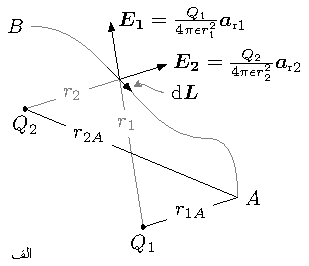
\includegraphics{figEnergyPotentialOfMultiplePointCharges}
\end{subfigure}%
%
\begin{subfigure}{0.5\textwidth}
\centering
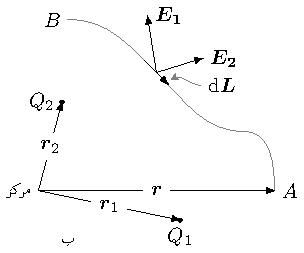
\includegraphics{figEnergyPotentialOfMultiplePointChargesNotAtOrigin}
\end{subfigure}%
\caption{دو نقطہ چارج کے میدان میں حتمی برقی دباو۔}
\label{شکل_توانائی_متعدد_نقطہ_چارج_دباو}
\end{figure}
%
\begin{align*}
\dif W&=-q \kvec{E} \cdot \dif \kvec{L}\\
&=-q (\kvec{E}_1+\kvec{E}_2) \cdot \dif \kvec{L}\\
&- \frac{q Q_1}{4\pi \epsilon_0 r_1^2} {\ar}_1 \cdot \dif \kvec{L}- \frac{q Q_2}{4\pi \epsilon_0 r_2^2} {\ar}_2 \cdot \dif \kvec{L}
\end{align*}
توانائی درکار ہو گی۔اس مساوات میں \عددیء{{\ar}_1 \cdot \dif \kvec{L}} حاصل کرتے وقت \عددیء{\dif \kvec{L}} کی قیمت مساوات \حوالہ{مساوات_توانائی_چھوٹا_فاصلہ_الف} سے لیتے ہوئے \عددیء{{\ar}_1 \cdot \dif \kvec{L}=\dif {r}_1} ملتا ہے۔اسی طرح \عددیء{{\ar}_2 \cdot \dif \kvec{L}} حاصل کرتے وقت \عددیء{\dif \kvec{L}} کی قیمت مساوات \حوالہ{مساوات_توانائی_چھوٹا_فاصلہ_ب} سے لیتے ہوئے \عددیء{{\ar}_2 \cdot \dif \kvec{L}=\dif {r}_2} ملتا ہے۔ان قیمتوں کے پُر کرنے سے
\begin{align*}
\dif W=- \frac{q Q_1 \dif r_1}{4\pi \epsilon_0 r_1^2} - \frac{q Q_2 \dif r_2}{4\pi \epsilon_0 r_2^2} 
\end{align*}
حاصل ہوتا ہے۔یوں \عددیء{B} سے \عددیء{A} تک کا پورا راستہ طے کرنے کی خاطر
\begin{align*}
W=\int_B^A \dif W&=- \frac{q Q_1 }{4\pi \epsilon_0} \int_{r_{1B}}^{r_{1A}} \frac{\dif r_1}{r_1^2} -\frac{q Q_2 }{4\pi \epsilon_0} \int_{r_{2B}}^{r_{2A}} \frac{\dif r_2}{r_2^2}\\
&=\frac{q Q_1 }{4\pi \epsilon_0} \left(\frac{1}{r_{1A}}-\frac{1}{r_{1B}} \right)+\frac{q Q_2 }{4\pi \epsilon_0} \left(\frac{1}{r_{2A}}-\frac{1}{r_{2B}} \right)
\end{align*}
توانائی درکار ہو گی۔نقطہ \عددیء{B} کو لامحدود فاصلے پر لیتے ہوئے یوں نقطہ \عددیء{A} پر حتمی برقی دباو
\begin{align}\label{مساوات_توانائی_نقطہ_چارج_کی_حتمی_دباو_پ}
V_A=\frac{W}{q}=\frac{1}{4\pi \epsilon_0} \left(\frac{Q_1}{r_{1A}}+\frac{Q_2}{r_{2A}} \right)
\end{align}
حاصل ہوتی ہے۔

مساوات \حوالہ{مساوات_توانائی_نقطہ_چارج_کی_حتمی_دباو_پ} میں دائیں ہاتھ پہلا جزو \عددیء{Q_1} کے میدان میں نقطہ \عددیء{ُA} کی حتمی برقی دباو جبکہ
 دوسرا جزو \عددیء{Q_2} کے میدان میں نقطہ \عددیء{ُA} کی حتمی برقی دباو دیتا ہے۔مساوات \حوالہ{مساوات_توانائی_نقطہ_چارج_کی_حتمی_دباو_پ}   کے مطابق \عددیء{Q_1} اور \عددیء{Q_2} دونوں کے موجودگی میں نقطہ \عددیء{A} کا برقی دباو حاصل کرنے کی خاطر ان دو چارجوں کو باری باری علیحدہ لیتے ہوئے \عددیء{A} پر برقی دباو حاصل کیا جاتا ہے اور پھر دونوں برقی دباو کا مجموعہ لیا جاتا ہے۔آپ دیکھ سکتے ہیں کہ یہی طریقہ کار دو سے زیادہ نقطہ چارجوں کے لئے بھی بروئے کار لایا جا سکتا ہے۔یوں کسی بھی نقطے کی برقی دباو حاصل کرتے ہوئے مختلف نقطہ چارجوں کے برقی دباو علیحدہ علیحدہ حاصل کرتے ہوئے انہیں جمع کرتے حاصل کیا جا سکتا ہے۔

اگر کسی کروی محدد کے مرکز سے \عددیء{Q_1} تک کا سمتیہ \عددیء{\kvec{r}_1} جبکہ مرکز سے \عددیء{Q_2} تک کا سمتیہ \عددیء{\kvec{r}_2} اور مرکز سے نقطہ \عددیء{A} تک سمتیہ \عددیء{\kvec{r}} ہوں تب  نقطہ \عددیء{A} کے لئے مساوات \حوالہ{مساوات_توانائی_نقطہ_چارج_کی_حتمی_دباو_پ} کو ہم یوں لکھ سکتے ہیں 
\begin{align}\label{مساوات_توانائی_نقطہ_چارج_کی_حتمی_دباو_ت}
V_A=\frac{1}{4\pi \epsilon_0} \left(\frac{Q_1}{\abs{\kvec{r}-\kvec{r}_1}}+\frac{Q_2}{\abs{\kvec{r}-\kvec{r}_2}} \right)
\end{align}
جہاں \عددیء{Q_1} سے \عددیء{A} تک فاصلہ \عددیء{\abs{\kvec{r}-\kvec{r}_1}} اور \عددیء{Q_2} سے \عددیء{A} تک  فاصلہ \عددیء{\abs{\kvec{r}-\kvec{r}_2}} ہے۔یہ صورت حال شکل \حوالہ{شکل_توانائی_متعدد_نقطہ_چارج_دباو}-ب میں دکھائی گئی ہے۔متعدد نقطہ چارجوں کے لئے مساوات \حوالہ{مساوات_توانائی_نقطہ_چارج_کی_حتمی_دباو_ت} 
\begin{gather}
\begin{aligned}\label{مساوات_توانائی_نقطہ_چارج_کی_حتمی_دباو_ٹ}
V(\kvec{r})&=\frac{1}{4\pi \epsilon_0} \left(\frac{Q_1}{\abs{\kvec{r}-\kvec{r}_1}}+\frac{Q_2}{\abs{\kvec{r}-\kvec{r}_2}}+\cdots+\frac{Q_n}{\abs{\kvec{r}-\kvec{r}_n}} \right)\\
&=\frac{1}{4\pi \epsilon_0} \sum_{j=1}^n \tfrac{Q_j}{\abs{\kvec{r}-\kvec{r}_j}}
\end{aligned}
\end{gather}
لکھی جائے گی  جہاں نقطہ \عددیء{A} کا مقام زیر نوشت میں \عددیء{A} لکھنے کی بجائے  \عددیء{V(\kvec{r})} میں \عددیء{\kvec{r}} سے  واضح کیا گیا ہے۔

متغیر حجمی چارج کثافت \عددیء{\rho_h} کے چھوٹے حجم \عددیء{\Delta h} میں پائے جانے والے  چارج \عددیء{\Delta Q=\rho_h \Delta h} کو نقطہ چارج تصور کیا جا سکتا ہے۔پورے حجم کے \عددیء{n} چھوٹے ٹکڑے کرتے ہوئے  مساوات \حوالہ{مساوات_توانائی_نقطہ_چارج_کی_حتمی_دباو_ٹ} کو یوں لکھا جا سکتا ہے
\begin{align}\label{مساوات_توانائی_نقطہ_چارج_کی_حتمی_دباو_ث}
V(\kvec{r})&=\frac{1}{4\pi \epsilon_0} \left(\frac{\rho_h(\kvec{r}_1) \Delta h_1}{\abs{\kvec{r}-\kvec{r}_1}}+\frac{\rho_h(\kvec{r}_2) \Delta h_2}{\abs{\kvec{r}-\kvec{r}_2}}+\cdots+\frac{\rho_h(\kvec{r}_n) \Delta h_n}{\abs{\kvec{r}-\kvec{r}_n}} \right)
\end{align}
جہاں \عددیء{\kvec{r}} کو کثافت کا آزاد متغیرہ لیتے ہوئے  مقام \عددیء{\kvec{r}_j} پر کثافت کو \عددیء{\rho_h(\kvec{r}_j)} اور چھوٹی حجم کو \عددیء{\Delta h_j} لکھا گیا ہے۔چھوٹی حجم \عددیء{\Delta h} کو کم سے کم  کرتے ہوئے ایسے نقطوں کی تعداد زیادہ سے زیادہ بناتے ہوئے اس مجموعہ سے مندرجہ ذیل حجمی تکمل حاصل ہوتا ہے۔
\begin{align}\label{مساوات_توانائی_نقطہ_چارج_کی_حتمی_دباو_ج}
V(\kvec{r})&=\int \limits_{\textup{حجم}} \frac{\rho_h(\kvec{r'}) \dif h'}{4\pi \epsilon_0\abs{\kvec{r}-\kvec{r}'}}
\end{align}

یہاں رک کر مندرجہ بالا مساوات کو دوبارہ دیکھتے ہیں۔\عددیء{\rho_h} حجمی چارج کثافت ہے۔مقام \عددیء{\kvec{r}'} پر چھوٹی حجم \عددیء{\dif h'} میں تھوڑا سا چارج \عددیء{\rho_h(\kvec{r}')\dif h'} پایا جاتا ہے جسے نقطہ چارج تصور کیا جاتا ہے۔مساوات \حوالہ{مساوات_توانائی_نقطہ_چارج_کی_حتمی_دباو_ج} نقطہ \عددیء{\kvec{r}} پر برقی دباو دیتا ہے جہاں برقی زمین کو لامحدود فاصلے پر تصور کیا گیا ہے۔یوں اکائی چارج کو لامحدود فاصلے سے نقطہ \عددیء{\kvec{r}} تک کسی بھی راستے لانے کے لئے اس مساوات سے حاصل \عددیء{V(\kvec{r})} برابر توانائی درکار ہو گی۔

اگر حجمی چارج کثافت کی جگہ سطحی چارج کثافت \عددیء{\rho_S} یا لکیری چارج کثافت \عددیء{\rho_L} پایا جاتا تب مندرجہ بالا مساوات کو
\begin{align}
V(\kvec{r})&=\int \limits_{\textup{سطح}} \frac{\rho_S(\kvec{r'}) \dif S'}{4\pi \epsilon_0\abs{\kvec{r}-\kvec{r}'}} \label{مساوات_توانائی_سطحی_دباو}\\
V(\kvec{r})&=\int \limits_{\textup{لکیر}} \frac{\rho_L(\kvec{r'}) \dif L'}{4\pi \epsilon_0\abs{\kvec{r}-\kvec{r}'}} \label{مساوات_توانائی_لکیری_دباو}
\end{align}
لکھتے۔ان مساوات میں \عددیء{\dif h'}، \عددیء{\dif S'} اور \عددیء{\dif L'} غیر سمتی یعنی مقداری ہیں۔تینوں اقسام کے چارج کثافت پائے جانے کی صورت میں باری باری ہر ایک سے پیدا برقی دباو حاصل کرتے ہوئے ان کا مجموعہ لیا جائے گا۔
%====================
\ابتدا{مثال}
\عددیء{z=0} سطح پر \عددیء{z} محدد کے گرد \عددیء{b} رداس کے گول دائرے پر \عددیء{\rho_L} چارج کثافت پایا جاتا ہے۔\عددیء{N(0,0,z)} پر برقی دباو حاصل کریں۔ 
\begin{figure}
\centering
\begin{subfigure}{0.5\textwidth}
\centering
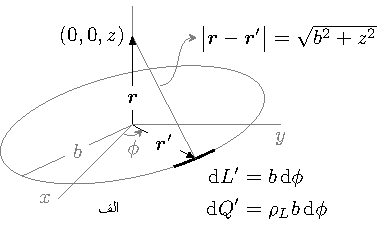
\includegraphics{figEnergyPotentialOfCircularChargeDensity}
\end{subfigure}%
%
\begin{subfigure}{0.5\textwidth}
\centering
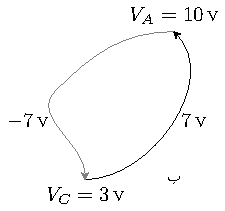
\includegraphics{figEnergyPotentialAroundLoopIsZero}
\end{subfigure}%
\caption{(الف) گول دائرے پر لکیری چارج کثافت سے \عددیء{z} محدد پر پیدا برقی دباو۔ (ب)بند دائرے کی برقی دباو صفر ہے۔}
\label{شکل_توانائی_گول_کثافت_برقی_دباو}
\end{figure}

حل:شکل \حوالہ{شکل_توانائی_گول_کثافت_برقی_دباو}-الف میں صورت حال دکھایا گیا ہے۔\عددیء{z=0} سطح پر کروی نظام کا رداس \عددیء{\kvec{r}} اور نلکی محدد کا رداس \عددیء{\kvec{\rho}} برابر ہوتے ہیں۔گول دائرے پہ \عددیء{\kvec{r}'} کے مقام پر چھوٹی لکیر  \عددیء{\dif L'=b \dif \phi} لکھی جا سکتی ہے۔برقی دباو \عددیء{\kvec{r}} پر درکار ہے۔شکل کو دیکھتے ہوئے مسئلہ فیثاغورث کی مدد سے \عددیء{\abs{\kvec{r}'-\kvec{r}}=\sqrt{b^2+z^2}} لکھا جا سکتا ہے۔یوں مساوات \حوالہ{مساوات_توانائی_لکیری_دباو} استعمال کرتے ہوئے نقطہ \عددیء{(0,0,z)} پر
\begin{align*}
V&=\int \limits_0^{2\pi} \frac{\rho_L b \dif \phi}{4\pi \epsilon_0 \sqrt{b^2+z^2}}=\frac{\rho_L b}{2 \epsilon_0 \sqrt{b^2+z^2}}
\end{align*}
برقی دباو پایا جائے گا۔گول دائرے کے عین  وسط یعنی \عددیء{(0,0,0)} پر یوں \عددیء{\tfrac{\rho_L}{2\epsilon_0}}  وولٹ کا برقی دباو پایا جائے گا۔
\انتہا{مثال}
%===================

مساوات \حوالہ{مساوات_دباو_لکیری_تکملہ} میں \عددیء{B} کو لامحدود فاصلے پر لیتے ہوئے کسی بھی دو نقطوں \عددیء{A} اور \عددیء{C} کے حتمی برقی دباو یوں لکھے جا سکتے ہیں۔
\begin{align*}
V_A&=-\int_{\infty}^{A} \kvec{E} \cdot \dif \kvec{L}\\
V_C&=-\int_{\infty}^{C} \kvec{E} \cdot \dif \kvec{L}
\end{align*}
شکل \حوالہ{شکل_توانائی_گول_کثافت_برقی_دباو}-ب میں یہ نقطے دکھائے گئے ہیں۔اب اگر \عددیء{V_A} دس وولٹ جبکہ \عددیء{V_C} تین وولٹ کے برابر ہو تب \عددیء{C} کے حوالے سے \عددیء{A} پر سات وولٹ ہوں گے یعنی  \عددیء{V_{AC}=\SI{7}{\volt}} ہو گا۔اسی طرح \عددیء{A} کے حوالے سے \عددیء{C} پر منفی سات وولٹ ہوں گے یعنی \عددیء{V_{CA}=\SI{-7}{\volt}} ہو گا۔یوں اگر کسی بھی راستے  \عددیء{C} سے \عددیء{A} جایا جائے تو برقی دباو میں سات وولٹ کا اضافہ ہو گا جبکہ کسی بھی راستے واپس \عددیء{C} لوٹنے سے برقی دباو میں سات وولٹ ہی کی کمی رونما ہو گی۔آپ دیکھ سکتے ہیں کہ کسی بھی نقطے سے شروع ہو کر بند دائرے پر چلتے ہوئے واپس اسی نقطے تک پہنچنے سے برقی دباو میں کُل کوئی تبدیلی پیدا نہیں ہو گی۔اس حقیقت کو یوں لکھا جاتا ہے
\begin{align*}
V_{AC}+V_{CA}=-\int_{C}^{A} \kvec{E} \cdot \dif \kvec{L}-\int_{A}^{C} \kvec{E} \cdot \dif \kvec{L}=0
\end{align*}
جہاں پہلے \عددیء{C} سے \عددیء{A} اور پھر \عددیء{A} سے واپس \عددیء{C} پہنچا گیا۔بند دائرے کے تکمل کو دو ٹکڑوں میں لکھنے کی بجائے اسے بند تکمل کی شکل میں لکھتے ہوئے اسی مساوات کو یوں بہتر لکھا جا سکتا ہے 
\begin{align}\label{مساوات_توانائی_بند_راستا}
\oint \kvec{E} \cdot \dif \kvec{L}=0
\end{align}
جہاں تکمل کے نشان پر گول دائرہ بند تکمل کو ظاہر کرتا ہے۔

مساوات \حوالہ{مساوات_توانائی_بند_راستا} کہتا ہے کہ کسی بھی طرح پیدا کئے گئے برقی میدان میں بند دائرے پر پورا چکر لگانے کے لئے صفر توانائی درکار ہوتی ہے۔حقیقت میں یہ مساوات صرف وقت کے ساتھ نہ تبدیل ہونے والے برقی میدان یعنی \اصطلاح{ساکن برقی میدان}\فرہنگ{ساکن برقی میدان}\حاشیہب{static electric field}\فرہنگ{static electric field}  کے لئے درست ہے۔اس کتاب میں وقت کے ساتھ بدلتے میدان پر بعد میں غور کیا جائے گا۔ایسے میدان جس میں بند دائرے پر چلنے کی خاطر کوئی توانائی درکار نہ ہو کو \اصطلاح{بقائی میدان}\فرہنگ{بقائی میدان}\حاشیہب{conservative field}\فرہنگ{conservative field} کہتے ہیں۔ساکن تجاذبی میدان بھی بقائی میدان\حاشیہد{یہ جملہ لکھنے کے ٹھیک ایک دن بعد نرگس مولولہ اور ان کے ساتھیوں نے تجاذبی موجیں دریافت کیں۔اس دریافت سے پہلے کسی بھی تجاذبی میدان کو بقائی میدان تصور کیا جاتا تھا۔آج سے ہم ساکن تجاذبی میدان کو ہی بقائی میدان کہیں گے۔} ہے۔یوں تجاذبی میدان میں پہاڑی کی چوٹی تک پہنچنے سے مخفی توانائی میں جتنا اضافہ پیدا ہو، چوٹی سے واپس اترنے پر مخفی توانائی میں اتنی ہی کمی رونما ہو گی اور یوں آپ کی ابتدائی اور اختتامی مخفی توانائی عین برابر ہوں گے۔

\begin{figure}
\centering
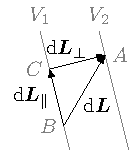
\includegraphics{figPotentialGradientIsField}
\caption{برقی دباو کی ڈھلوان برقی میدان ہے۔}
\label{شکل_توانائی_دباو_ڈھلوان_میدان_ہے}
\end{figure}

\حصہ{برقی دباو کی ڈھلوان}
شکل \حوالہ{شکل_توانائی_دباو_ڈھلوان_میدان_ہے} میں دو انتہائی قریب  ہم قوہ  سطحیں دکھائی گئی ہیں جن پر \عددیء{V_1} اور \عددیء{V_2} برقی دباو پایا جاتا ہے۔ہم قوہ سطح \عددیء{V_1} پر کسی نقطہ  \عددیء{B} سے ہم قوہ سطح \عددیء{V_2} پر کسی نقطہ \عددیء{A} تک  کا سمتی فاصلہ \عددیء{\dif \kvec{L}} لیتے ہوئے \عددیء{B} سے \عددیء{A}  تک حرکت کرنے سے برقی دباو میں  \عددیء{-\kvec{E} \cdot \dif \kvec{L}} تبدیلی رونما ہو گی جہاں برقی میدان کو \عددیء{\kvec{E}} لکھا گیا ہے۔
\begin{align}\label{مساوات_توانائی_ہم_قوہ_سطح_اور_میدان}
\dif V=V_2-V_1=-\kvec{E} \cdot \dif \kvec{L}
\end{align}
چھوٹی لمبائی \عددیء{\dif \kvec{L}} پر برقی میدان کو غیر تغیر پذیر تصور کیا جا سکتا ہے۔چونکہ  دو نقطوں کے مابین برقی دباو کا ابتدائی نقطے سے اختتامی نقطے پہنچنے کے راستے پر منحصر نہیں ہوتا لہٰذا ہم \عددیء{B} سے \عددیء{C} اور پھر \عددیء{A} بھی جا سکتے تھے۔\عددیء{B} سے \عددیء{C} تک فاصلے کو \عددیء{\dif \kvec{L}_\parallel}  جبکہ \عددیء{C} سے \عددیء{A} تک فاصلے کو \عددیء{\dif \kvec{L}_\perp}  لکھتے ہوئے
\begin{align}
\dif V=-\kvec{E} \cdot (\dif \kvec{L}_\parallel+ \dif \kvec{L}_\perp)
\end{align}
لکھا جا سکتا ہے۔\عددیء{\kvec{E}} کو  ہم قوہ سطحہ کے متوازی  اور اس کے عمودی اجزاء کی صورت میں یوں لکھا جا سکتا ہے
\begin{align}
\kvec{E}=\kvec{E}_\parallel+\kvec{E}_\perp
\end{align}  
جس سے
\begin{align}
\dif V=-(\kvec{E}_\parallel+\kvec{E}_\perp) \cdot (\dif \kvec{L}_\parallel+ \dif \kvec{L}_\perp)=-{E}_\parallel \dif L_\parallel-E_\perp \dif L_\perp
\end{align}  
حاصل ہوتا ہے جہاں \عددیء{\kvec{E}_\parallel} اور \عددیء{\dif \kvec{L}_\parallel} کے مابین صفر درجے کا زاویہ ہونے کی بنا پر 
 \عددیء{\kvec{E}_\parallel \cdot \dif \kvec{L}_\parallel=E_\parallel \dif L_\parallel} لکھا گیا ہے جبکہ \عددیء{\kvec{E}_\parallel} اور
 \عددیء{\dif \kvec{L}_\perp} کے مابین نوے درجے کا زاویہ ہونے کی بنا پر \عددیء{\kvec{E}_\parallel \cdot \dif \kvec{L}_\perp=0} ہے۔اس مساوات کا پہلا جزو \عددیء{-{E}_\parallel \dif L_\parallel} نقطہ \عددیء{B} اور \عددیء{C} کے درمیان برقی دباو دیتا ہے۔ہم قوہ سطح پر ہر جگہ برابر برقی دباو پایا جاتا ہے لہٰذا \عددیء{B} اور \عددیء{C} کے درمیان کسی قسم کا برقی دباو نہیں پایا جاتا یعنی \عددیء{-{E}_\parallel \dif L_\parallel} صفر کے برابر ہے۔اب چونکہ \عددیء{\dif L_\parallel} صفر کے برابر نہیں ہے لہٰذا کسی بھی ہم قوہ سطح پر
\begin{align}
\kvec{E}_\parallel=0
\end{align}
ہو گا اور سطح پر صرف اور صرف عمودی برقی میدان پایا جائے گا یعنی
\begin{align}
\kvec{E}=\kvec{E}_\perp
\end{align}
یوں
\begin{align}
\dif V=-E_\perp \dif L_\perp
\end{align}  
لکھا جا سکتا ہے۔یہ ذہن میں رکھتے ہوئے کہ ہم قوہ سطح پر صرف عمودی میدان پایا جاتا ہے، مندرجہ بالا مساوات میں \عددیء{\kvec{E}_\perp} کی جگہ \عددیء{\kvec{E}} لکھتے ہیں۔
\begin{align}
\dif V=-E \dif L_\perp
\end{align}
اس مساوات سے
\begin{align}
E=-\frac{\dif V_{\phantom{\perp}}}{\dif L_\perp}
\end{align}
حاصل ہوتا ہے جہاں سے ظاہر ہے کہ \عددیء{E} درحقیقت \عددیء{V} کے ڈھلوان کے برابر مگر الٹ سمت میں ہے۔یوں
\begin{align}
\kvec{E}=-\frac{\dif V_{\phantom{\perp}}}{\dif L_\perp} 
\end{align}
لکھا جا سکتا ہے جہاں \عددیء{\kvec{a}_N} ہم قوہ سطح کا عمودی اکائی سمتیہ ہے۔

کسی نقطہ کو برقی زمین تصور کرتے ہوئے کسی دوسرے نقطے کی برقی دباو کو حتمی برقی دباو تصور کیا جاتا ہے جو نقطے کے مقام پر منحصر ہوتا ہے لہٰذا اسے \عددیء{V(x,y,z)} لکھا جا سکتا ہے جہاں برقی دباو کے آزاد متغیرات \عددیء{x}، \عددیء{y} اور \عددیء{z} ہیں۔کسی بھی قابو متغیرہ کی طرح \عددیء{V(x,y,z)} کا تفرق
\begin{align}\label{مساوات_توانائی_دباو_کارتیسی_تفرق}
\dif V=\frac{\partial V}{\partial x} \dif x+\frac{\partial V}{\partial y} \dif y +\frac{\partial V}{\partial z} \dif z
\end{align}
لکھا جا سکتا ہے۔کارتیسی محدد میں کسی بھی برقی دباو کو
\begin{align}\label{مساوات_توانائی_میدان}
\kvec{E}=E_x \ax+ E_y \ay+E_z \az
\end{align}
اور  چھوٹی لمبائی کو
\begin{align}\label{مساوات_توانائی_کارتیسی_چھوٹا_فاصلہ}
\dif \kvec{L}=\dif x \ax+\dif y \ay+\dif z \az
\end{align}
لکھا جا سکتا ہے۔یہاں آپ صفحہ \حوالہصفحہ{مساوات_سمتیہ_کارتیسی_چھوٹا_فاصلہ} پر دئے مساوات \حوالہ{مساوات_سمتیہ_کارتیسی_چھوٹا_فاصلہ} پر دوبارہ نظر ڈال سکتے ہیں۔مندرجہ بالا تین مساوات کو مساوات \حوالہ{مساوات_توانائی_ہم_قوہ_سطح_اور_میدان} میں پُر کرتے ہوئے
\begin{align}\label{مساوات_توانائی_دباو_اور_میدان}
\frac{\partial V}{\partial x} \dif x+\frac{\partial V}{\partial y} \dif y +\frac{\partial V}{\partial z} \dif z=-E_x \dif x-E_y \dif y-E_z \dif z
\end{align}
حاصل ہوتا ہے۔\عددیء{y} اور \عددیء{z} تبدیل کئے بغیر (یعنی \عددیء{\dif y=0} اور \عددیء{\dif z=0} لیتے ہوئے) \عددیء{x} تبدیل کرنے سے اس مساوات کے بائیں اور دائیں ہاتھ کا پہلا جزو یعنی \عددیء{\frac{\partial V}{\partial x} \dif x} اور \عددیء{-E_x \dif x} تبدیل ہوتے ہیں لہٰذا یہ لازم ہے کہ یہ دونوں اجزاء برابر ہوں یعنی \عددیء{\tfrac{\partial V}{\partial x} \dif x=-E_x \dif x} جس سے \عددیء{E_x=-\tfrac{\partial V}{\partial x}} حاصل ہوتا ہے۔اگر \عددیء{\frac{\partial V}{\partial x} \dif x} اور \عددیء{-E_x \dif x} برابر نہ ہوں تب مساوات کے ایک طرف تبدیلی دوسرے طرف کے تبدیلی کے برابر نہیں ہو گی اور یوں مساوات کے دونوں اطراف برابر نہیں رہیں گے۔اسی طرح صرف \عددیء{y} اور صرف \عددیء{z} تبدیل کئے جا سکتا ہیں۔یوں
\begin{gather}
\begin{aligned}
E_x&=-\frac{\partial V}{\partial x}\\
E_y&=-\frac{\partial V}{\partial y}\\
E_z&=-\frac{\partial V}{\partial z}
\end{aligned}
\end{gather}
لکھا جا سکتا ہے جسے مساوت \حوالہ{مساوات_توانائی_میدان} میں پُر کرتے
\begin{align}\label{مساوات_توانائی_ڈھلوان_تعریف_الف}
\kvec{E}=-\left( \frac{\partial V}{\partial x} \ax+\frac{\partial V}{\partial y} \ay+\frac{\partial V}{\partial z} \az\right)
\end{align}
لکھا جا سکتا ہے۔

اگر ہم
\begin{align}\label{مساوات_توانائی_ڈھلوان_تعریف_ب}
\nabla=\frac{\partial }{\partial x} \ax+\frac{\partial }{\partial y} \ay+\frac{\partial }{\partial z} \az \quad \quad \textrm{کارتیسی محدد میں ڈھلوان کی مساوات}
\end{align} 
لکھیں جہاں کسی بھی مقداری \عددیء{f} کے لئے \عددیء{\nabla f} سے مراد \عددیء{ \tfrac{\partial f}{\partial x} \ax+\tfrac{\partial f}{\partial y} \ay+\tfrac{\partial f}{\partial z} \az} ہو تب مندرجہ بالا مساوات کو
\begin{align}\label{مساوات_توانائی_ڈھلوان_تعریف_پ}
\kvec{E}=-\nabla V
\end{align}
لکھا جا سکتا ہے۔\عددیء{\nabla V} کو برقی دباو کی \اصطلاح{ڈھلوان}\فرہنگ{ڈھلوان}\حاشیہب{gradient}\فرہنگ{gradient} پڑھا جاتا ہے۔مساوات \حوالہ{مساوات_توانائی_ڈھلوان_تعریف_ب} کا بایاں ہاتھ ڈھلوان کی علامت جبکہ اس کا دایاں ہاتھ ڈھلوان کے عمل کو ظاہر کرتا ہے۔اگرچہ ہم نے ڈھلوان کا عمل برقی دباو اور برقی میدان کے لئے حاصل کیا، حقیقت میں یہ عمل سائنس کے دیگر متغیرات کے لئے بھی درست ثابت ہوتا ہے۔اس کی مقبولیت اسی حقیقت کی وجہ سے ہے کہ یہ جگہ جگہ پیش آتا ہے۔ڈھلوان کا عمل مقداری پر کیا جاتا ہے جبکہ اس کا حاصل جواب سمتیہ ہوتا ہے۔صفحہ \حوالہصفحہ{مساوات_گاوس_پھیلاو} پر مساوات \حوالہ{مساوات_گاوس_پھیلاو} پھیلاو کی تعریف بیان کرتا ہے جہاں پھیلاو کا عمل سمتیہ پر کرتے ہوئے مقداری\حاشیہد{طلباء و طالبات  عموماً ڈھلوان کے حاصل جواب کے اکائی سمتیات کو غائب کرتے ہوئے انہیں پھیلاو کے ساتھ منسلک کر لیتے ہیں۔ایسا کرنے سے گریز کریں۔ } حاصل کی جاتی ہے۔پھیلاو کے اس مساوات کو یہاں موازنے کے لئے دوبارہ پیش کرتے ہیں۔
\begin{align}
\nabla \cdot \kvec{D}=\frac{\partial D_x}{\partial x}+\frac{\partial D_y}{\partial y}+\frac{\partial D_z}{\partial z}
\end{align}
%===============
\ابتدا{مشق}
تفاعل \عددیء{f(x,y,z)=3+z^2 e^{y}\sin x} کا ڈھلوان حاصل کریں۔

جواب: \عددیء{z^2 e^y \cos x \ax+z^2 e^y \sin x \ay+2 z e^y \sin x \az}
\انتہا{مشق}
%===================

\ابتدا{مثال}\شناخت{مثال_توانائی_ڈھلوان_مختلف_نقطوں_کے_متغیرات_کے_ساتھ}
نقطہ \عددیء{N_1(x_1,y_1,z_1)} سے نقطہ \عددیء{N_2(x_2,y_2,z_2)} کا سمتی فاصلہ \عددیء{\kvec{R}_{21}=(x_2-x_1)\ax+(y_2-y_1)\ay+(z_2-z_1)\az} ہے جبکہ ان کے مابین فاصلہ \عددیء{R_{21}=\sqrt{(x_2-x_1)^2+(y_2-y_1)^2+(z_2-z_1)^2}}  ہے۔نقطہ \عددیء{N_2} پر \عددیء{\tfrac{1}{R_{21}}} کی ڈھلوان  حاصل کریں۔

حل:نقطہ \عددیء{N_2} پر ڈھلوان حاصل کرتے وقت \عددیء{x_2}، \عددیء{y_2} اور \عددیء{z_2} کو متغیرات تصور کیا جاتا ہے جبکہ \عددیء{x_1}، \عددیء{y_1} اور \عددیء{z_1} کو اٹل قیمتیں تصور کیا جاتا ہے۔یوں ڈھلوان کی تعریف
\begin{align*}
\nabla_2 =\frac{\partial }{\partial x_2} \ax+\frac{\partial }{\partial y_2} \ay+\frac{\partial }{\partial z_2} \az 
\end{align*}
لکھی جائے گی جہاں \عددیء{\nabla_2} کے زیر نوشت میں \عددیء{2} یاد دہانی کراتا ہے کہ نقطہ \عددیء{N_2} کے متغیرات ڈھلوان حاصل کرتے ہوئے استعمال کئے جائیں گے۔ڈھلوان کا پہلا جزو
\begin{align*}
\frac{\partial }{\partial x_2} \frac{1}{R_{21}} &=\frac{\partial }{\partial x_2}[(x_2-x_1)^2+(y_2-y_1)^2+(z_2-z_1)^2]^{-\frac{1}{2}}\\
&=-\frac{1}{2} [(x_2-x_1)^2+(y_2-y_1)^2+(z_2-z_1)^2]^{-\frac{3}{2}} \left[2(x_2-x_1)\right]\\
&=\frac{-(x_2-x_1)}{ [(x_2-x_1)^2+(y_2-y_1)^2+(z_2-z_1)^2]^{\frac{3}{2}}}
\end{align*}
یعنی
\begin{align*}
\frac{\partial }{\partial x_2} \frac{1}{R_{21}} &=\frac{-(x_2-x_1)}{R_{21}^3}
\end{align*}
حاصل ہوتا ہے۔بقایا دو اجزاء بھی بالکل اسی طرح حل کرتے ہوئے
\begin{align*}
\nabla_2 \frac{1}{R_{21}} =\frac{-(x_2-x_1)\ax-(y_2-y_1)\ay-(z_2-z_1)\az}{R_{21}^3}
\end{align*}
یعنی
\begin{align}\label{مساوات_توانائی_فاصلہ_ڈھلوان}
\nabla_2 \frac{1}{R_{21}} =-\frac{\kvec{R}_{21}}{R_{21}^3}=-\frac{\kvec{a}_{R21}}{R_{21}^2}
\end{align}
لکھا جا سکتا ہے۔
\انتہا{مثال}
%====================
\ابتدا{مشق}
مندرجہ بالا مساوات میں نقطہ \عددیء{N_2} پر ڈھلوان حاصل کی گئی۔اب آپ نقطہ \عددیء{N_1} پر \عددیء{\tfrac{1}{R_{21}}} کی ڈھلوان حاصل کرتے ہوئے ثابت کریں کہ
\begin{align}
\nabla_1 \frac{1}{R_{21}} =\frac{\kvec{R}_{21}}{R_{21}^3}
\end{align}
کے برابر ہے۔یوں 
\begin{align}\label{مساوات_توانائی_فاصلے_کی_ڈھلوان_ب}
\nabla_1 \frac{1}{R_{21}}=-\nabla_2 \frac{1}{R_{21}}
\end{align}
لکھا جا سکتا ہے۔
\انتہا{مشق}
%=================

\جزوحصہ{نلکی محدد میں ڈھلوان}
نلکی محدد میں برقی دباو کے آزاد متغیرات نلکی محدد کے متغیرات ہوں گے اور یوں برقی دباو \عددیء{V(\rho,\phi,z)} لکھا جائے گا۔مساوات \حوالہ{مساوات_توانائی_دباو_کارتیسی_تفرق}، مساوات \حوالہ{مساوات_توانائی_میدان} اور مساوات \حوالہ{مساوات_توانائی_کارتیسی_چھوٹا_فاصلہ} کو نلکی محدد میں یوں لکھ سکتے ہیں

\begin{align}
\dif V&=\frac{\partial V}{\partial \rho} \dif \rho+\frac{\partial V}{\partial \phi} \dif \phi +\frac{\partial V}{\partial z} \dif z \label{مساوات_توانائی_دباو_نلکی_تفرق}\\
\kvec{E}&=E_\rho \arho+ E_\phi \aphi+E_z \az \label{مساوات_توانائی_نلکی_میدان}\\
\dif \kvec{L}&=\dif \rho \arho+\rho \dif \phi \aphi+\dif z \az \label{مساوات_توانائی_نلکی_چھوٹا_فاصلہ}
\end{align}
جہاں چھوٹی لمبائی \عددیء{\dif \kvec{L}} کو صفحہ \حوالہصفحہ{مساوات_سمتیہ_نلکی_چھوٹا_فاصلہ} پر مساوات \حوالہ{مساوات_سمتیہ_نلکی_چھوٹا_فاصلہ} کی مدد سے لکھا گیا ہے۔
مندرجہ بالا تین مساوات کو مساوات \حوالہ{مساوات_توانائی_ہم_قوہ_سطح_اور_میدان} میں پُر کرتے ہوئے
\begin{align}
\frac{\partial V}{\partial \rho} \dif \rho+\frac{\partial V}{\partial \phi} \dif \phi +\frac{\partial V}{\partial z} \dif z=-\left(E_\rho \dif \rho+E_\phi \rho \dif \phi+E_z \dif z\right)
\end{align}
حاصل ہوتا ہے۔\عددیء{\phi} اور \عددیء{z} تبدیل کئے بغیر (یعنی \عددیء{\dif \phi=0} اور \عددیء{\dif z=0} لیتے ہوئے) \عددیء{\rho} تبدیل کرنے سے  اس مساوات کے بائیں اور دائیں ہاتھ کا پہلا جزو یعنی \عددیء{\tfrac{\partial V}{\partial \rho} \dif \rho} اور \عددیء{-E_\rho \dif \rho}  تبدیل ہوتے ہیں۔ اگر یہ اجزاء ہر صورت برابر رہیں صرف اور صرف اسی صورت مندرجہ بالا مساوات کے دونوں بازو برابر رہیں گے لہٰذا \عددیء{-E_\rho \dif \rho=\tfrac{\partial V}{\partial \rho} \dif \rho} ہو گا جس سے \عددیء{E_\rho=-\tfrac{\partial V}{\partial \rho} } حاصل ہوتا ہے۔اسی طرح باری باری \عددیء{\phi} اور \عددیء{z} تبدیل کرتے ہوئے
\begin{align*}
E_\phi \rho \dif \phi&=-\frac{\partial V}{\partial \phi} \dif \phi\\
E_z \dif z&=-\frac{\partial V}{\partial z} \dif z
\end{align*}
لکھے جا سکتے ہیں جس سے \عددیء{E_\phi} اور \عددیء{E_z} کے مساوات حاصل ہوتے ہیں۔ان تمام جوابات کو یکجا کرتے ہیں۔
\begin{gather}
\begin{aligned}
E_\rho&=-\frac{\partial V}{\partial \rho}\\
E_\phi &=-\frac{1}{\rho}\frac{\partial V}{\partial \phi} \\
E_z &=-\frac{\partial V}{\partial z} 
\end{aligned}
\end{gather}
انہیں مساوات \حوالہ{مساوات_توانائی_نلکی_میدان} میں پُر کرتے ہوئے
\begin{align}
\kvec{E}=-\left( \frac{\partial V}{\partial \rho} \arho+\frac{1}{\rho}\frac{\partial V}{\partial \phi}  \aphi+\frac{\partial V}{\partial z}\az \right)
\end{align}
حاصل ہوتا ہے۔اس کو مساوات \حوالہ{مساوات_توانائی_ڈھلوان_تعریف_پ} کی شکل میں لکھتے ہوئے نلکی محدد میں ڈھلوان کی مساوات
\begin{align}\label{مساوات_توانائی_ڈھلوان_نلکی}
\nabla = \frac{\partial }{\partial \rho} \arho+\frac{1}{\rho}\frac{\partial }{\partial \phi}  \aphi+\frac{\partial }{\partial z}\az \quad \quad \textrm{نلکی محدد میں ڈھلوان کی مساوات}
\end{align}
حاصل ہوتی ہے۔مساوات \حوالہ{مساوات_توانائی_ڈھلوان_تعریف_ب} اور مساوات \حوالہ{مساوات_توانائی_ڈھلوان_نلکی} کا موازنہ کریں۔کارتیسی محدد کی مساوات نسبتاً آسان ہے۔
 
\جزوحصہ{کروی محدد میں ڈھلوان}
صفحہ \حوالہصفحہ{مساوات_سمتیہ_کروی_چھوٹا_فاصلہ} پر مساوات \حوالہ{مساوات_سمتیہ_کروی_چھوٹا_فاصلہ} کروی محدد میں چھوٹی لمبائی \عددیء{\dif \kvec{L}} کی مساوات ہے۔کروی محدد میں کسی بھی نقطے کے برقی دباو کو \عددیء{V(r,\theta\phi)} لکھا جا سکتا ہے جبکہ کسی بھی سمتیہ کی طرح \عددیء{\kvec{E}} کو تین عمودی حصوں میں لکھا جا سکتا ہے۔یوں ہم مساوات \حوالہ{مساوات_توانائی_دباو_کارتیسی_تفرق}، مساوات \حوالہ{مساوات_توانائی_میدان} اور مساوات \حوالہ{مساوات_توانائی_کارتیسی_چھوٹا_فاصلہ} کو کروی محدد میں یوں لکھ سکتے ہیں۔
\begin{align}
\dif V&=\frac{\partial V}{\partial r} \dif r+\frac{\partial V}{\partial \theta} \dif \theta +\frac{\partial V}{\partial \phi} \dif \phi \\
\kvec{E}&=E_r \ar+ E_\theta \atheta+E_\phi \aphi \label{مساوات_توانائی_کروی_میدان_سمتیہ}\\
\dif \kvec{L}&=\dif r \ar+r \dif \theta \atheta+r \sin \theta \dif \phi \aphi
\end{align}
ان تین مساوات کو مساوات \حوالہ{مساوات_توانائی_ہم_قوہ_سطح_اور_میدان} میں پُر کرتے ہوئے

\begin{align}
\frac{\partial V}{\partial r} \dif r+\frac{\partial V}{\partial \theta} \dif \theta +\frac{\partial V}{\partial \phi} \dif \phi=-\left(E_r \dif r+E_\theta r \dif \theta +E_\phi r \sin \theta \dif \phi  \right)
\end{align}
حاصل ہوتا ہے۔اب اگر ہم صرف \عددیء{r} کو تبدیل کریں تب \عددیء{\dif \theta=0} اور \عددیء{\dif \phi=0} ہوں گے لہٰذا مندرجہ بالا مساوات کے بائیں دائیں بازو کا پہلا جزو یعنی \عددیء{\tfrac{\partial V}{\partial r} \dif r} اور \عددیء{-E_r \dif r} تبدیل ہوں گے۔یہ اجزاء بالکل برابر ہونے کی صورت میں ہی مساوات کے دونوں بازو برابر رہیں گے لہٰذا ہم \عددیء{\tfrac{\partial V}{\partial r} \dif r=-E_r \dif r} لکھ سکتے ہیں جس سے  \عددیء{E_r=-\tfrac{\partial V}{\partial r}} حاصل ہوتا ہے۔اسی طرح باری باری \عددیء{} اور \عددیء{} تبدیل کرتے ہوئے مساوات کے دونوں بازو کے اجزاء برابر لکھتے ہوئے
\begin{align*}
\frac{\partial V}{\partial \theta} \dif \theta &=-E_\theta r \dif \theta \\
\frac{\partial V}{\partial \phi} \dif \phi&=-E_\phi r \sin \theta \dif \phi
\end{align*}
حاصل ہوتا ہے جس سے \عددیء{E_\theta} اور \عددیء{E_\phi} کے مساوات حاصل ہوتے ہیں۔ان تمام جوابات کو یکجا کرتے ہیں۔
\begin{align*}
E_r&=-\frac{\partial V}{\partial r}\\
E_\theta &=-\frac{1}{r}\frac{\partial V}{\partial \theta}  \\
E_\phi &=-\frac{1}{r \sin \theta}\frac{\partial V}{\partial \phi}
\end{align*}
ان قیمتوں کو مساوات \حوالہ{مساوات_توانائی_کروی_میدان_سمتیہ} میں پُر کرتے ہوئے
\begin{align}\label{مساوات_توانائی_کروی_ڈھلوان_سے_میدان}
\kvec{E}=-\left(\frac{\partial V}{\partial r} \ar+\frac{1}{r}\frac{\partial V}{\partial \theta}\atheta+\frac{1}{r \sin \theta}\frac{\partial V}{\partial \phi} \aphi \right)
\end{align}
لکھا جا سکتا ہے جس سے کروی محدد میں ڈھلوان کی مساوات یوں لکھی جا سکتی ہے۔
 \begin{align}
\nabla=\frac{\partial }{\partial r} \ar+\frac{1}{r}\frac{\partial }{\partial \theta}\atheta+\frac{1}{r \sin \theta}\frac{\partial }{\partial \phi} \aphi \quad \quad \textrm{کروی محدد میں ڈھلوان کی مساوات}
\end{align}
%==============

\ابتدا{مشق}
صفحہ \حوالہصفحہ{حصہ_گاوس_عمومی_پھیلاو} پر حصہ \حوالہ{حصہ_گاوس_عمومی_پھیلاو} میں پھیلاو کی عمومی مساوات کا حصول دکھایا گیا جہاں عمومی محدد کے متغیرات \عددیء{(u,v,w)} اور اکائی سمتیات \عددیء{(\au, \av, \aw)} لئے گئے۔ایسا ہی کرتے ہوئے ڈھلوان کی عمومی مساوات حاصل کریں۔

جواب:
\begin{align*}
\nabla=\frac{1}{K_1} \frac{\partial }{\partial u} \au+\frac{1}{K_2} \frac{\partial }{\partial v} \av+\frac{1}{K_3} \frac{\partial }{\partial w} \aw \quad \quad \textrm{ڈھلوان کی عمومی مساوات}
\end{align*}
\انتہا{مشق}
%=============================
\ابتدا{مثال}
صفحہ \حوالہ{مساوات_توانائی_نقطہ_چارج_کی_حتمی_دباو_الف} پر مساوات \حوالہ{مساوات_توانائی_نقطہ_چارج_کی_حتمی_دباو_الف} نقطہ چارج کا برقی دباو دیتا ہے۔مساوات \حوالہ{مساوات_توانائی_کروی_ڈھلوان_سے_میدان} کے استعمال سے کروی محدد میں \عددیء{\kvec{E}} کی مساوات حاصل کریں۔

حل:برقی دباو \عددیء{V=\tfrac{Q}{4\pi \epsilon_0 r}} کروی محدد کے رداس پر منحصر ہے جبکہ \عددیء{\theta} اور \عددیء{\phi} کا اس میں کوئی کردار نہیں لہٰذا مساوات \حوالہ{مساوات_توانائی_کروی_ڈھلوان_سے_میدان} میں \عددیء{\tfrac{\partial V}{\partial \theta}} اور \عددیء{\tfrac{\partial V}{\partial \phi}} صفر کے برابر ہوں گے۔اس طرح \عددیء{\tfrac{\partial V}{\partial r}} لیتے ہوئے \عددیء{\kvec{E}=\tfrac{Q}{4\pi \epsilon_0 r^2}\ar} حاصل ہوتا ہے۔
\انتہا{مثال}
%=====================

یہاں بتلاتا چلوں کہ حقیقی دنیا میں عموماً برقی دباو معلوم ہوتی ہے جس سے برقی میدان کا حصول درکار ہوتا ہے۔اس کی مثال بجلی کی دو تاریں ہو سکتی ہیں جن کے درمیان \عددیء{\SI{220}{\volt}} پایا جاتا ہے اور جن کے درمیان آپ برقی میدان جاننا چاہتے ہوں۔

\حصہ{جفت قطب}
شکل \حوالہ{شکل_توانائی_جفت_قطب}-الف میں محدد کے مرکز سے \عددیء{\tfrac{d}{2}} فاصلے پہ \عددیء{z} محدد پر ایک جانب \عددیء{+Q} اور دوسری جانب \عددیء{-Q} نقطہ چارج دکھائے گئے ہیں۔یوں برابر مقدار مگر الٹ علامت کے نقطہ چارجوں کے درمیان \عددیء{d} فاصلہ ہے۔ایسی جوڑی چارجوں کو \اصطلاح{جفت قطب}\فرہنگ{جفت قطب}\حاشیہب{dipole}\فرہنگ{dipole} کہا جاتا ہے۔ہمیں جفت قطب سے دور نقطہ \عددیء{N} پر برقی میدان اور برقی دباو کی قیمتیں درکار ہیں۔کسی بھی دور نقطے سے یہ دونوں چارج تقریباً مرکز پر دکھائی دیتے ہیں۔دور نقطے سے ایسا نقطہ مراد ہے جہاں مرکز سے نقطے تک کا فاصلہ \عددیء{r} جفت قطب چارجوں کے درمیان فاصلہ \عددیء{d} سے بہت زیادہ ہو یعنی جب \عددیء{r\gg d} ہو۔ہم دیکھ سکتے ہیں کہ \عددیء{r} یا \عددیء{\theta} تبدیل کرنے سے برقی میدان تبدیل ہو گا جبکہ \عددیء{\phi} تبدیل کرنے سے ایسا نہیں ہو گا۔شکل \حوالہ{شکل_توانائی_جفت_قطب}-الف میں \عددیء{R_1} اور \عددیء{R_2} دونوں \عددیء{r} کی جانب جھک  کر \عددیء{N} پر آ ملتے ہیں۔نقطہ \عددیء{N} کو جتنا دور لے جایا جائے اتنی ہی \عددیء{R_1} اور \عددیء{R_2} دونوں  \عددیء{r}  کے  متوازی صورت اختیار کرتے ہیں حتٰی کہ آخر کار یہ شکل \حوالہ{شکل_توانائی_جفت_قطب}-ب کی طرح نظر آتے ہیں۔آئیں اس شکل کی مدد سے دور نقطے پر برقی دباو اور برقی میدان حاصل کریں۔

\begin{figure}
\centering
\begin{subfigure}{0.5\textwidth}
\centering
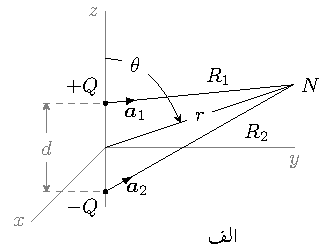
\includegraphics{figEnergyDipole}
\end{subfigure}%
%
\begin{subfigure}{0.5\textwidth}
\centering
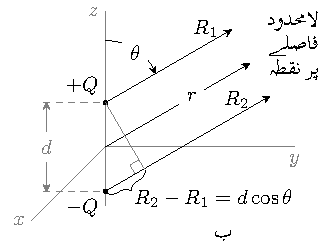
\includegraphics{figEnergyDipoleFieldAtInfinity}
\end{subfigure}%
\caption{جفت قطب}
\label{شکل_توانائی_جفت_قطب}
\end{figure}

شکل \حوالہ{شکل_توانائی_جفت_قطب}-ب میں \عددیء{R_1}، \عددیء{R_2} اور  \عددیء{r} تینوں \عددیء{z} محدد کے ساتھ \عددیء{\theta} زاویہ بناتے ہیں۔چارج \عددیء{+Q} سے \عددیء{R_2} پر عمود بناتے ہوئے
\begin{gather}
\begin{aligned}\label{مساوات_توانائی_جفت_قطب_فاصلوں_میں_فرق}
R_2-R_1&=d \cos \theta \\
R_1 & =r-\frac{d}{2} \cos \theta\\
R_2 & =r+\frac{d}{2} \cos \theta
\end{aligned}
\end{gather}
لکھا جا سکتا ہے۔شکل \حوالہ{شکل_توانائی_جفت_قطب}-الف میں \عددیء{N} پر برقی دباو \عددیء{V} مساوات \حوالہ{مساوات_توانائی_نقطہ_چارج_کی_حتمی_دباو_ت} کی مدد سے
\begin{align}\label{مساوات_توانائی_جفت_قطب_دباو_بنیادی_مساوات}
V=\frac{1}{4\pi \epsilon_0} \left(\frac{Q}{R_1}-\frac{Q}{R_2}\right)=\frac{Q}{4\pi \epsilon_0} \left(\frac{R_2-R_1}{R_1 R_2}\right)
\end{align}
لکھی جا سکتی ہے۔مساوات \حوالہ{مساوات_توانائی_جفت_قطب_فاصلوں_میں_فرق} کی مدد سے اسے
\begin{align*}
V&=\frac{Q}{4\pi \epsilon_0} \frac{d \cos \theta}{(r-\frac{d}{2} \cos \theta)(r+\frac{d}{2} \cos \theta)}\\
&=\frac{Q}{4\pi \epsilon_0} \frac{d \cos \theta}{(r^2-\frac{d^2}{4} \cos^2 \theta)}\\
&=\frac{Q}{4\pi \epsilon_0 r^2} \frac{d \cos \theta}{(1-\frac{d^2}{4 r^2} \cos^2 \theta)}
\end{align*}
لکھا جا سکتا ہے۔نیچے قوسین میں \عددیء{\cos \theta \le 1} اور \عددیء{r\gg d} کی وجہ سے \عددیء{1\gg\frac{d^2}{4 r^2} \cos^2 \theta} ہو گا اور یوں \عددیء{\frac{d^2}{4 r^2} \cos^2 \theta} کو نظرانداز کیا جا سکتا ہے۔یوں
\begin{align}\label{مساوات_توانائی_جفت_قطب_دباو}
V=\frac{Qd \cos \theta}{4\pi \epsilon_0 r^2}
\end{align} 
حاصل ہوتا ہے۔مساوات \حوالہ{مساوات_توانائی_کروی_ڈھلوان_سے_میدان} کو استعمال کرتے ہوئے اس مساوات سے برقی میدان لکھتے ہیں۔
\begin{align}\label{مساوات_توانائی_جفت_قطب_دور_میدان_الف}
\kvec{E}=\frac{Q d}{4\pi \epsilon_0 r^3}\left(2 \cos \theta \ar+\sin \theta \atheta \right)
\end{align}

ہم پہلے برقی دباو اور پھر ڈھلوان کی مدد سے برقی میدان حاصل کرنے کے بجائے پہلے برقی میدان اور پھر تکمل استعمال کرتے ہوئے برقی دباو حاصل کر سکتے ہیں البتہ ایسا کرنا اتنا آسان ثابت نہیں ہوتا۔شوق رکھنے والوں کے لئے مثال \حوالہ{مثال_توانائی_جفت_قطب} میں اسی طریقے کو استعمال کرتے ہوئے دور نقطے پر جفت قطب  سے پیدا میدان اور برقی دباو حاصل کئے گئے ہیں۔

جفت قطب کا چارج \عددیء{\abs{Q}} ضرب چارجوں کے درمیان سمتی فاصلہ \عددیء{\kvec{d}} کو \اصطلاح{معیار اثر جفت قطب}\فرہنگ{جفت قطب!معیار اثر}\حاشیہب{dipole moment}\فرہنگ{dipole moment}  کہتے ہیں اور اسے \عددیء{\kvec{p}} سے ظاہر کیا جاتا ہے۔یوں 
\begin{align}\label{مساوات_توانائی_سمتی_جفت_قطب}
\kvec{p}=Q \kvec{d}
\end{align}
کے برابر ہے جہاں سمتی فاصلہ منفی چارج سے مثبت چارج کی سمت میں ہوتا ہے لہٰذا شکل \حوالہ{شکل_توانائی_جفت_قطب} میں \عددیء{\kvec{d}=d \az} ہے۔اس طرح چونکہ \عددیء{\az \cdot \ar=\cos \theta} کے برابر ہے لہٰذا یوں ہم مساوات \حوالہ{مساوات_توانائی_جفت_قطب_دباو} کو
\begin{align}
V=\frac{\kvec{p} \cdot \ar}{4 \pi \epsilon_0 r^2}
\end{align} 

لکھ سکتے ہیں۔ اسی مساوات کو مزید یوں بھی لکھا جا سکتا ہے
\begin{align}
V=\frac{1}{4\pi \epsilon_0 \abs{\kvec{r}-\kvec{r}'}^2} \kvec{p} \cdot \frac{\kvec{r}-\kvec{r}'}{\abs{\kvec{r}-\kvec{r}'}}
\end{align}
جہاں \عددیء{\kvec{r}} اس نقطے کی نشاندہی کرتا ہے جہاں برقی دباو حاصل کیا جا رہا ہو جبکہ \عددیء{\kvec{r}'} جفت قطب کے مرکز کی نشاندہی کرتا ہے۔یہ مساوات کسی بھی محدد نظام سے آزاد مساوات ہے۔

مساوات \حوالہ{مساوات_توانائی_جفت_قطب_دباو} کے تحت \عددیء{r} بڑھانے سے  برقی دباو \عددیء{r^2} گنا کم ہوتا ہے۔یاد رہے کہ اکیلے چارج کا برقی دباو ایسی صورت میں \عددیء{r} گنا کم ہوتا ہے۔ہمیں تعجب نہیں ہونا چاہیے چونکہ دور سے جفت قطب کے دو چارج نہایت قریب قریب نظر آتے ہیں جس سے مثبت چارج کا اثر منفی چارج کا اثر تقریباً ختم کرتا ہے۔یہی حقیقت مساوات \حوالہ{مساوات_توانائی_جفت_قطب_دور_میدان_الف} میں بھی نظر آتا ہے جہاں \عددیء{r} بڑھانے سے  \عددیء{\kvec{E}} کی قیمت \عددیء{r^3} گنا کم ہوتی ہے۔

جب تک \عددیء{Q} ضرب \عددیء{\kvec{d}} کی قیمت تبدیل نہ ہو اس وقت تک دور کسی بھی نقطے پر جفت قطب کے اثرات میں کوئی تبدیلی رونما نہیں ہوتی۔یوں \عددیء{Q} کو کم  یا زیادہ کرتے ہوئے اگر \عددیء{\kvec{d}} کو یوں تبدیل کیا جائے کہ \عددیء{Q \kvec{d}} تبدیل نہ ہو تو جفت قطب سے دور نقطے پر جفت قطب کے اثرات میں کوئی تبدیلی نہیں پائی جائے گی۔اب اگر  ہم \عددیء{Q \kvec{d}} کی قیمت محدود رکھتے ہوئے  \عددیء{\kvec{d}} کو اتنا کم کر دیں کہ اسے صفر تصور  کیا جا سکے  اور ساتھ ہی ساتھ \عددیء{Q} کو اتنا بڑھا دیں کہ اسے لامحدود تصور کیا جا سکے  تو ایسی صورت میں ہمیں \اصطلاح{نقطہ جفت قطب}\فرہنگ{جفت قطب! نقطہ} حاصل ہو گا۔


\جزوحصہ{جفت قطب کے سمت بہاو خط}
ہم پہلے صفحہ \حوالہصفحہ{حصہ_کولومب_سمت_بہاو_خط} پر حصہ \حوالہ{حصہ_کولومب_سمت_بہاو_خط} میں \اصطلاح{سمت بہاو خط}\فرہنگ{خط!سمت بہاو}\حاشیہب{streamlines}\فرہنگ{streamlines} پر غور کر  چکے ہیں۔آئیں جفت قطب کے سمت بہاو خط کھینچنا دیکھیں۔برقی دباو کے سمت بہاو خط مساوات \حوالہ{مساوات_توانائی_جفت_قطب_دباو} کی مدد سے کھینچے جا سکتے ہیں۔اس مساوات میں \عددیء{\tfrac{Qd}{4\pi \epsilon_0}} مستقل ہے جسے ایک کے برابر لیتے ہوئے  \عددیء{V=\tfrac{\cos \theta}{r^2}} حاصل ہوتا ہے۔مختلف برقی دباو کی قیمتوں کے لئے اسے کھینچ کر برقی دباو کے سمت بہاو خط حاصل کئے جاتے ہیں۔شکل \حوالہ{شکل_توانائی_جفت_قطب_ہم_قوہ_اور_سمت_بہاو_خط} میں \عددیء{V=0.2,0.4,0.6,0.8} کے لئے اس مساوات کے خط دکھائے گئے ہیں۔ مساوات \حوالہ{مساوات_توانائی_جفت_قطب_دباو_بنیادی_مساوات} کے تحت دونوں چارج سے برابر فاصلہ پر \عددیء{V=0} حاصل ہوتا ہے۔یوں \عددیء{z=0} لامحدود سطح پر برقی دباو صفر ہو گا اور یہ بطور برقی زمین کردار ادا کرے گی۔ 

جفت قطب کے میدان کے سمت بہاو خط مساوات \حوالہ{مساوات_توانائی_جفت_قطب_دور_میدان_الف} کی مدد سے کھینچے جاتے ہیں۔اس مساوات کا پہلا جزو کسی بھی نقطے پر \عددیء{\ar} سمت میں میدان \عددیء{E_r} دیتا ہے جبکہ اس کا دوسرا جزو اسی نقطے پر \عددیء{\atheta} سمت میں میدان \عددیء{E_\theta} دیتا ہے۔اس طرح اس نقطے پر ہم
\begin{align*}
\frac{E_r}{E_\theta}=\frac{\dif r}{r \dif \theta} =\frac{2 \cos \theta}{\sin \theta}
\end{align*}
یا
\begin{align*}
\frac{\dif r}{r } =\frac{2 \cos \theta}{\sin \theta}\dif \theta
\end{align*}
لکھ کر تکمل لیتے ہوئے
\begin{align*}
\ln r =2 \ln \sin \theta +\ln M
\end{align*}
یا
\begin{align}
r=M \sin^2 \theta
\end{align}
حاصل کرتے ہیں جہاں \عددیء{\ln M} تکمل کا مستقل ہے۔یہ مساوات جفت قطب کے میدان کے سمت بہاو خط دیتا ہے جنہیں شکل \حوالہ{شکل_توانائی_جفت_قطب_ہم_قوہ_اور_سمت_بہاو_خط} میں \عددیء{M=1,1.5,2,2.5} کے لئے کھینچا گیا ہے۔برقی زمین پر برقی میدان عمودی ہے۔
\begin{figure}
\centering
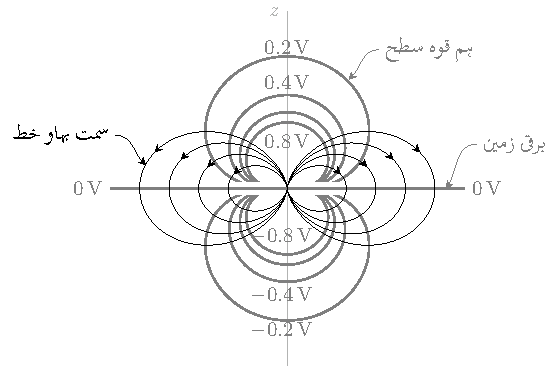
\includegraphics{figEnergyDipoleEquipotentialLines}
\caption{جفت قطب کے ہم قوہ اور سمت بہاو خط۔}
\label{شکل_توانائی_جفت_قطب_ہم_قوہ_اور_سمت_بہاو_خط}
\end{figure}
%=================

\ابتدا{مثال}\شناخت{مثال_توانائی_جفت_قطب}
شکل \حوالہ{شکل_توانائی_جفت_قطب}-الف میں دکھائے گئے جفت قطب سے دور کسی نقطے \عددیء{N} پر پہلے برقی میدان اور پھر اس برقی میدان کو استعمال کرتے ہوئے برقی دباو حاصل کریں۔

صفحہ \حوالہصفحہ{مثال_سمتیہ_جفت_قطب} پر مثال \حوالہ{مثال_سمتیہ_جفت_قطب} میں \عددیء{\kvec{R}_1=R_1 \kvec{a}_{1}} اور
 \عددیء{\kvec{R}_2=R_2\kvec{a}_{2}} سمتیوں کو کروی نظام میں لکھنا دکھایا گیا ہے۔ انہیں یہاں دوبارہ پیش کرتے ہیں۔
\begin{align*}
\kvec{R}_1 &=(r-\frac{d}{2}\cos\theta)\ar+\frac{d}{2}\sin\theta \atheta\\
\kvec{R}_2 &=(r+\frac{d}{2}\cos \theta )\ar-\frac{d}{2}\sin \theta \atheta
\end{align*}
جس سے \عددیء{R_1=\abs{\kvec{R}_1}=\sqrt{\kvec{R}_1 \cdot \kvec{R}_1}} حاصل کرتے ہیں۔
\begin{gather}
\begin{aligned}\label{مساوات_توانائی_جفت_قطب_فاصلے}
R_1&=\sqrt{\left(r-\frac{d}{2}\cos\theta\right)^2+\left(\frac{d}{2}\sin\theta \atheta \right)^2}\\
&=r \sqrt{1-\frac{d}{r} \cos \theta +\frac{d^2}{r^2}}\\
&\approx r \sqrt{1-\frac{d}{r} \cos \theta } \quad \quad (d \ll r)
\end{aligned}
\end{gather}
آخری قدم پر \عددیء{d \ll r} کی بنا پر \عددیء{\tfrac{d^2}{r^2}} کو رد کیا گیا ہے۔ہم جانتے ہیں کہ
\begin{align*}
(a+b)^n=a^n +\frac{n a^{n-1}b}{1!}+\frac{n(n-1)a^{n-2}b^2}{2!}+\cdots
\end{align*}
لکھا جا سکتا ہے۔اگر \عددیء{a=1} اور \عددیء{b=-\tfrac{d}{r} \cos \theta} کے برابر ہوں تب مساوات \حوالہ{مساوات_توانائی_جفت_قطب_فاصلے} میں دئے \عددیء{R_1} کی طاقت تین کے لئے ہم لکھ سکتے ہیں
\begin{align*}
R_1^3=r^3 (1-\tfrac{d}{r} \cos \theta)^{\frac{3}{2}}=r^3 \left( 1-\tfrac{3d}{2 r} \cos \theta+\cdots \right)
\end{align*}
اس مساوات کے پہلے دو جزو دکھائے گئے ہیں۔اس کے تیسرے جزو میں \عددیء{\tfrac{d^3}{r^3}}چوتھے جزو میں \عددیء{\tfrac{d^4}{r^4}} پائے جاتے ہیں  لہٰذا پہلے دو اجزاء کے علاوہ تمام اجزاء کو نظرانداز کیا جا سکتا ہے۔یوں
\begin{align}
R_1^3=r^3 \left(1-\frac{3d}{2r} \cos \theta\right)
\end{align}
صورت اختیار کر لیتا ہے۔یہی عمل \عددیء{R_2^3} کے لئے کرنے سے
\begin{align}
R_2^3=r^3 \left(1+\frac{3d}{2r} \cos \theta\right)
\end{align}
حاصل ہوتا ہے۔صفحہ \حوالہصفحہ{مساوات_کولومب_قوت_کی_عمومی_مساوات} پر مساوات \حوالہ{مساوات_کولومب_قوت_کی_عمومی_مساوات} کو استعمال کرتے ہوئے دونوں چارجوں سے کُل برقی میدان ان کے علیحدہ علیحدہ میدان کے مجموعہ لے کو یوں لکھا جا سکتا ہے۔
\begin{align*}
\kvec{E}&=\frac{Q}{4\pi\epsilon_0} \frac{\kvec{R}_1}{R_1^3}-\frac{Q}{4\pi\epsilon_0} \frac{\kvec{R}_2}{R_2^3}\\
&=\frac{Q}{4\pi\epsilon_0}\left(\frac{\left[(r-\frac{d}{2}\cos\theta)\ar+\frac{d}{2}\sin\theta \atheta\right]}{r^3 (1-\frac{3d}{2r} \cos \theta)}-\frac{\left[(r+\frac{d}{2}\cos \theta )\ar-\frac{d}{2}\sin \theta \atheta\right]}{r^3 (1+\frac{3d}{2r} \cos \theta)} \right)\\
&=\frac{Qd }{4\pi\epsilon_0 r^3}\left( \frac{2 \cos \theta \ar+\sin \theta \atheta}{(1-\frac{3d}{2r} \cos \theta)(1+\frac{3d}{2r} \cos \theta)}\right)
\end{align*}
اس مساوات میں کسر کے نچلے حصے کو ضرب دیتے ہوئے \عددیء{(1-\tfrac{9d^2}{4r^2}\cos^2\theta \approx 1)} لکھا جا سکتا ہے جہاں \عددیء{\tfrac{d^2}{r^2}} والے جزو کو نظرانداز کیا گیا ہے۔یوں
\begin{align}\label{مساوات_توانائی_جفت_قطب_دور_میدان_ب}
\kvec{E}=\frac{Qd }{4\pi\epsilon_0 r^3}( 2 \cos \theta \ar+\sin \theta \atheta)
\end{align}
حاصل ہوتا ہے جو مساوات \حوالہ{مساوات_توانائی_جفت_قطب_دور_میدان_الف} ہی ہے۔

آئیں اب مساوات \حوالہ{مساوات_توانائی_جفت_قطب_دور_میدان_ب} سے نقطہ \عددیء{N_0(r,\theta,\phi)} پر برقی دباو حاصل کریں۔ہم برقی زمین کو لامحدود فاصلے پر رکھتے ہیں۔ لامحدود فاصلے پر نقطہ  \عددیء{N_3(\infty,\theta',\phi')} سے کروی محدد کے مرکز کی جانب سیدھا چلتے ہوئے ہم پہلے \عددیء{N_2(r,\theta',\phi')} تک پہنچتے ہیں۔اس کے بعد صرف \عددیء{\theta} تبدیل کرتے ہوئے ہم \عددیء{N_1(r,\theta,\phi')} پہنچیں گے اور آخر کار \عددیء{r} اور \عددیء{\theta} تبدیل کئے بغیر \عددیء{N_0(r,\theta,\phi)} پہنچیں گے۔  

صفحہ \حوالہصفحہ{مساوات_سمتیہ_کروی_چھوٹا_فاصلہ} پر مساوات \حوالہ{مساوات_سمتیہ_کروی_چھوٹا_فاصلہ} کروی محدد میں چھوٹی لمبائی \عددیء{\dif \kvec{L}} کی مساوات ہے۔اسے یہاں دوبارہ لکھتے ہیں۔
\begin{align}
\dif \kvec{L}=\dif r \ar+r \dif \theta \atheta+r\sin \theta \dif \phi \aphi
\end{align}
\عددیء{N_3} سے \عددیء{N_2} تک چلتے ہوئے \عددیء{\dif \theta=0} اور \عددیء{\dif \phi=0} ہوں گے لہٰذا \عددیء{N_3} کے حوالے سے \عددیء{N_2} پر برقی دباو \عددیء{V_{23}}
\begin{align*}
V_{23}&=-\int_{N_3}^{N_2} \kvec{E} \cdot \dif \kvec{L}=-\frac{Qd }{4\pi\epsilon_0}\int_{N_3}^{N_2} \frac{( 2 \cos \theta \ar+\sin \theta \atheta)\cdot \dif r \ar}{r^3} \\
&=-\frac{Qd }{4\pi\epsilon_0}\int_{N_3}^{N_2} \frac{ 2 \cos \theta  \dif r }{r^3}=\left .\frac{Q d \cos \theta}{4 \pi \epsilon_0 r^2}\right|_{\infty,\theta',\phi'}^{r,\theta',\phi'}=\frac{Q d \cos \theta'}{4 \pi \epsilon_0 r^2}
\end{align*}
حاصل ہوتا ہے۔اب \عددیء{N_2} سے \عددیء{N_1} چلتے ہیں۔ہم اس راستے \عددیء{\dif r=0} اور \عددیء{\dif \phi=0} رکھتے ہیں لہٰذا
\begin{align*}
V_{12}&=-\int_{N_2}^{N_1} \kvec{E} \cdot \dif \kvec{L}=-\frac{Qd }{4\pi\epsilon_0}\int_{N_2}^{N_1} \frac{( 2 \cos \theta \ar+\sin \theta \atheta)\cdot  r \dif \theta \atheta}{r^3}  \\
&=-\frac{Qd }{4\pi\epsilon_0}\int_{N_2}^{N_1} \frac{\sin \theta  \dif \theta}{r^2}=\left. \frac{Qd }{4\pi\epsilon_0} \frac{\cos \theta}{r^2}\right|_{r,\theta',\phi'}^{r,\theta,\phi'}=\frac{Qd }{4\pi\epsilon_0} \frac{(\cos \theta-\cos \theta')}{r^2}
\end{align*} 
ہو گا۔اب \عددیء{N_1} سے \عددیء{N} چلتے ہیں۔اس راستے \عددیء{\dif r=0} اور \عددیء{\dif \theta=0} رکھے گئے ہیں لہٰذا
\begin{align*}
V_{01}&=-\int_{N_1}^{N_0} \kvec{E} \cdot \dif \kvec{L}=-\frac{Qd }{4\pi\epsilon_0}\int_{N_1}^{N_0} \frac{( 2 \cos \theta \ar+\sin \theta \atheta)\cdot  r \sin \theta \dif \phi \aphi}{r^3}=0
\end{align*} 
حاصل ہوتا ہے جہاں \عددیء{\ar \cdot \aphi=0} اور \عددیء{\atheta \cdot \aphi=0} کی بدولت تکمل صفر کے برابر لیا گیا ہے۔یوں \عددیء{V_{23}}، \عددیء{V_{12}} اور \عددیء{V_{01}} جمع کرتے ہوئے \عددیء{N_3} سے \عددیء{N_0} تک کا برقی دباو
\begin{align}
V_{0}=V_{03}=V_{23}+V_{12}+V_{01}=\frac{Qd \cos \theta}{4 \pi \epsilon_0 r^2}
\end{align}

حاصل ہوتا ہے جو مساوات \حوالہ{مساوات_توانائی_جفت_قطب_دباو} ہی ہے۔
\انتہا{مثال}
%==========

مندرجہ بالا مثال سے آپ نے دیکھ لیا ہو گا کہ پہلے برقی میدان اور بعد میں برقی دباو حاصل کرنا زیادہ مشکل کام ہے۔برقی دباو کی افادیت  اس مثال سے صاف ظاہر ہے۔حقیقی دنیا میں عموماً برقی دباو ہی  معلوم ہوتی ہے جیسے دو متوازی دھاتی چادروں کے درمیان برقی دباو یا گھریلو صارفین کے ہاں دو برقی تاروں کے درمیان برقی دباو۔ہم ایسی برقی دباو جانتے ہوئے اس سے مختلف متغیرات حاصل کرتے ہیں۔ 
%===========

\حصہ{ساکن برقی میدان کی کثافت توانائی}
برقی دباو پر غور کرتے ہوئے ہم نے دیکھا کہ برقی میدان میں لامحدود فاصلے سے چارج کو کسی نقطہ منتقل کرنے کے لئے توانائی درکار ہوتی ہے۔یہ توانائی چارج کو حرکت دینے والا محرک مہیا کرتا ہے۔چونکہ توانائی اٹل ہے لہٰذا یہ توانائی بصورت مخفی توانائی چارج میں منتقل ہو جاتی ہے۔جب تک بیرونی قوت چارج کو اس نقطے پر روکے رکھے یہ توانائی چارج میں بطور مخفی توانائی رہے گی۔اگر چارج کو بیرونی طاقت نہ روکے تو مخفی توانائی \اصطلاح{حرکی}\فرہنگ{حرکی توانائی}\حاشیہب{kinetic energy}\فرہنگ{kinetic energy} توانائی میں تبدیل ہوتے ہوئے چارج کو حرکت دے گی۔یوں اب چارج ازخود کام کرنے کے قابل ہو گا۔

آئیں دیکھیں کہ اگر اسی طرح مختلف چارج کو لامحدود فاصلے سے مختلف مقامات پر لا کر وہیں روکے رکھا جائے تو اس پورے نظام کی کُل مخفی توانائی کتنی ہو گی۔یہ توانائی ان چارجوں کو اپنی اپنی  جگہوں پر منتقل کرنے کے لئے درکار بیرونی توانائی کے مجموعے سے حاصل کی جا سکتی ہے۔

شروع خالی خلاء سے کرتے ہیں۔خالی خلاء میں چونکہ کوئی چارج نہیں پایا جاتا لہٰذا اس میں برقی میدان صفر کے برابر ہو گا۔یوں پہلے چارج \عددیء{Q_1} کو لامحدود فاصلے سے  نقطہ \عددیء{N_1} منتقل کرنے کے لئے صفر توانائی درکار ہو گی۔اب چونکہ خلاء میں \عددیء{Q_1} موجود ہے لہٰذا دوسرے چارج \عددیء{Q_2} کو  نقطہ \عددیء{N_2} منتقل کرنے کے لئے \عددیء{Q_2 V_{2,1}} توانائی درکار ہو گی جہاں \عددیء{N_2} پر پہلے چارج کی وجہ سے پیدا برقی دباو کو \عددیء{V_{2,1}} لکھا گیا ہے۔\عددیء{V_{2,1}} لکھتے ہوئے زیر نوشت میں پہلا عدد منتقل کئے جانے والے چارج کی نشاندہی کرتا ہے جبکہ پہلا عدد  منتقلی کے نقطے پر برقی دباو پیدا کرنے والے چارج کی نشاندہی کرتا ہے۔یوں
\begin{align*}
\textup{\RL{چارج $Q_2$ منتقل کرنے کے لئے درکار توانائی}}=Q_2 V_{2,1}
\end{align*}
لکھا جائے گا۔اب خلاء میں دو عدد چارج پائے جاتے ہیں لہٰذا  نقطہ \عددیء{N_3} پر \عددیء{Q_1} سے پیدا \عددیء{V_{3,1}} اور \عددیء{Q_2} سے پیدا \عددیء{V_{3,2}} برقی دباو ہوں گے۔یوں \عددیء{N_3} پر کل \عددیء{V_{3,1}+V_{3,2}} برقی دباو ہو گا لہٰذا
\begin{align*}
\textup{\RL{چارج $Q_3$ منتقل کرنے کے لئے درکار توانائی}}=Q_3 V_{3,1} +Q_3 V_{3,2}
\end{align*}
اور اسی طرح
\begin{align*}
\textup{\RL{چارج $Q_4$ منتقل کرنے کے لئے درکار توانائی}}=Q_4 V_{4,1} +Q_4 V_{4,2}+Q_4 V_{4,3}
\end{align*}
ہو گا۔یہی طریقہ کار مزید چارج منتقل کرنے کے لئے درکار توانائی دریافت کرنے کے لئے استعمال کیا جائے گا۔کل مخفی توانائی \عددیء{W} تمام چارجوں کو منتقل کرنے کے لئے درکار توانائی کے برابر ہو گا جو مندرجہ بالا طرز کے تمام جوابات کا مجموعہ ہو گا یعنی
\begin{gather}
\begin{aligned}\label{مساوات_توانائی_چارج_کثافت_توانائی_الف}
W&=Q_2 V_{2,1}+Q_3 V_{3,1} +Q_3 V_{3,2}+Q_4 V_{4,1} +Q_4 V_{4,2}+Q_4 V_{4,3}+\cdots\\
&=Q_2(V_{2,1})+Q_3( V_{3,1}+V_{3,2})+Q_4(V_{4,1} +V_{4,2}+V_{4,3})+\cdots
\end{aligned}
\end{gather}
مندرجہ بالا مساوات میں کسی رکن مثلاً \عددیء{Q_4 V_{4,2}} کو دیکھیں۔ اسے یوں
\begin{align*}
Q_4 V_{4,2} = Q_4 \frac{Q_2}{4\pi \epsilon_0 R_{42}}= Q_2 \frac{Q_4}{4\pi \epsilon_0 R_{24}}= Q_2 V_{2,4}
\end{align*}
 لکھا جا سکتا ہے جہاں \عددیء{Q_2} اور \عددیء{Q_4} کے درمیان مقداری فاصلے کو \عددیء{R_{42}} یا \عددیء{R_{24}} لکھا جا سکتا ہے۔اس طرح \عددیء{Q_4 V_{4,2}} کو \عددیء{Q_2 V_{2,4}} لکھا جا سکتا ہے۔اس طرح مساوات \حوالہ{مساوات_توانائی_چارج_کثافت_توانائی_الف} کے ہر جزو کو تبدیل کرتے ہوئے اسے
\begin{gather}
\begin{aligned}\label{مساوات_توانائی_چارج_کثافت_توانائی_ب}
W&=Q_1 V_{1,2}+Q_1 V_{1,3} +Q_2 V_{2,3}+Q_1 V_{1,4} +Q_2 V_{2,4}+Q_3 V_{3,4}+\cdots\\
&=Q_1 (V_{1,2}+V_{1,3} + V_{1,4} +\cdots)+Q_2 (V_{2,3}+V_{2,4}+\cdots)+Q_3(V_{3,4}+\cdots)
\end{aligned}
\end{gather}
  لکھا جا سکتا ہے۔مساوات \حوالہ{مساوات_توانائی_چارج_کثافت_توانائی_الف} اور مساوات \حوالہ{مساوات_توانائی_چارج_کثافت_توانائی_ب} کو جمع کرتے ہوئے
\begin{gather}
\begin{aligned}
2 W=\phantom{+}&Q_1(V_{1,2}+V_{1,3} + V_{1,4} +\cdots)\\
+&Q_2 (V_{2,1}+V_{2,3}+V_{2,4}+\cdots)\\
+&Q_3( V_{3,1}+V_{3,2}+V_{3,4}+\cdots)\\
+&\cdots
\end{aligned}
\end{gather}
حاصل ہوتا ہے۔اس مساوات کے پہلے قوسین میں \عددیء{V_{1,2}} نقطہ \عددیء{N_1} پر \عددیء{Q_2} کا پیدا کردہ برقی دباو ہے۔اسی طرح \عددیء{V_{1,3}} نقطہ \عددیء{N_1} پر \عددیء{Q_3} کا پیدا کردہ برقی دباو ہے جبکہ \عددیء{V_{1,4}} یہیں پر \عددیء{Q_4} کا پیدا کردہ برقی دباو ہے۔یوں قوسین میں بند قیمت نقطہ \عددیء{N_1} پر تمام چارجوں کا مجموعی برقی دباو \عددیء{V_1} ہے۔یاد رہے کہ \عددیء{N_1} پر برقی دباو حاصل کرتے وقت یہیں پر پائے جاتے چارج \عددیء{Q_1} کو شامل نہیں کیا جاتا۔یوں
\begin{align*}
V_1=V_{1,2}+V_{1,3} + V_{1,4} +\cdots
\end{align*}

کے برابر ہے۔اس طرح مندرجہ بالا مساوات سے
\begin{align}\label{مساوات_توانائی_چارج_کثافت_توانائی_پ}
W=\frac{1}{2}\left(Q_1 V_1+Q_2 V_2+Q_3 V_3+\cdots\right)=\frac{1}{2}\sum_{m=1}^{n} Q_m V_m
\end{align}
حاصل ہوتا ہے جہاں 
\begin{align*}
V_1&=V_{1,2}+V_{1,3} + V_{1,4} +\cdots\\
V_2&=V_{2,1}+V_{2,3}+V_{2,4}+\cdots\\
V_3&=V_{3,1}+V_{3,2}+V_{3,4}+\cdots
\end{align*}
لکھے گئے ہیں۔

ایسی حجم جس میں حجمی چارج کثافت \عددیء{\rho_h} پائی جائے کی کل مخفی توانائی حاصل کرنے کی غرض سے  چھوٹے چھوٹے حجم \عددیء{\dif h} میں چارج \عددیء{\dif Q=\rho_h \dif h} کو نقطہ چارج تصور کرتے ہوئے مساوات \حوالہ{مساوات_توانائی_چارج_کثافت_توانائی_پ} کا استعمال کیا جا سکتا ہے۔ایسی صورت میں یہ مساوات تکمل کی شکل اختیار کر لے گی یعنی
 \begin{align}\label{مساوات_توانائی_کثافت_تونائی}
W=\frac{1}{2}\int \limits_h \rho_h V \dif h
\end{align}
جہاں تکمل پورے حجم \عددیء{h} کے لئے حاصل کیا گیا ہے۔

مثال \حوالہ{مثال_توانائی_توانائی_ضرب_برقی_بہاو_کی_ڈھلوان} میں کارتیسی محدد استعمال کرتے ہوئے مندرجہ ذیل مساوات کا ثبوت دکھایا گیا ہے۔
\begin{align}\label{مساوات_توانائی_توانائی_ضرب_برقی_بہاو_کی_ڈھلوان}
\nabla \cdot  (V \kvec{D})=V (\nabla \cdot \kvec{D})+\kvec{D} \cdot (\nabla V)
\end{align}
مساوات \حوالہ{مساوات_توانائی_توانائی_ضرب_برقی_بہاو_کی_ڈھلوان} اور  صفحہ \حوالہصفحہ{مساوات_گاوس_میکسویل_پہلی_مساوات_نقطہ_شکل} پر مساوات \حوالہ{مساوات_گاوس_میکسویل_پہلی_مساوات_نقطہ_شکل} کے استعمال سے مساوات \حوالہ{مساوات_توانائی_کثافت_تونائی} کو یوں لکھا جا سکتا ہے۔
\begin{gather}
\begin{aligned}\label{مساوات_توانائی_کا_تکمل}
W&=\frac{1}{2}\int\limits_h (\nabla \cdot \kvec{D} )V \dif h\\
&=\frac{1}{2} \int \limits_h [\nabla \cdot (V \kvec{D})-\kvec{D} \cdot (\nabla V)] \dif h
\end{aligned}
\end{gather}
اس مساوات میں تکمل کے دو اجزاء ہیں۔پہلے جزو کو مسئلہ پھیلاو، جسے صفحہ \حوالہصفحہ{مساوات_گاوس_مسئلہ_پھیلاو_تکمل_شکل} پر مساوات \حوالہ{مساوات_گاوس_مسئلہ_پھیلاو_تکمل_شکل}  دیتا ہے، کی مدد سے بند سطحی تکمل کی صورت میں یوں لکھا جا سکتا ہے۔
\begin{align}\label{مساوات_توانائی_لامحدود_سطح_بند_تکمل_صفر}
\frac{1}{2}\int\limits_h \nabla \cdot (V \kvec{D}) \dif h = \frac{1}{2}\oint \limits_S (V \kvec{D}) \cdot \dif \kvec{S}
\end{align} 
یہاں بائیں جانب حجم \عددیء{h} جبکہ دائیں جانب اس حجم کی سطح \عددیء{S} پر تکمل حاصل کیا جاتا ہے۔\عددیء{h} اس حجم کو ظاہر کرتا ہے جس میں مساوات \حوالہ{مساوات_توانائی_کثافت_تونائی} کے تمام چارج پائے جاتے ہیں۔مساوات \حوالہ{مساوات_توانائی_کثافت_تونائی} میں حجم کے ایسے حصے بھی ہوں گے جہاں چارج کثافت \عددیء{\rho_h} کی قیمت صفر ہو گی۔ایسے حصوں کا تکمل \عددیء{\rho_h=0} کی بنا پر صفر کے برابر ہو گا۔یوں اگر حجم کو لامحدود کر دیا جائے تب بھی تکمل کی قیمت وہی رہے گی چونکہ ایسی اضافی حجم میں  \عددیء{\rho_h=0} ہو گا۔مساوات \حوالہ{مساوات_توانائی_لامحدود_سطح_بند_تکمل_صفر} میں یوں حجم کو لامحدود لیا جا سکتا ہے۔لامحدود حجم کو گھیرتی سطح کو کرہ شکل کا تصور کرتے ہوئے ایسی سطح \عددیء{4 \pi r^2} کے برابر ہو گی جہاں \عددیء{r \to \infty} ہو گا۔لامحدود رداس کی سطح سے دیکھتے ہوئے کسی بھی شکل کا چارج کثافت نقطہ مانند چارج \عددیء{Q} نظر آئے گا جو سطح پر \عددیء{D=\tfrac{Q}{4\pi r^2}} میدان اور \عددیء{V=\tfrac{Q}{4\pi \epsilon_0 r}} برقی دباو پیدا کرے گا۔ یوں مساوات \حوالہ{مساوات_توانائی_لامحدود_سطح_بند_تکمل_صفر}  کے دائیں جانب بند تکمل رداس کے ساتھ \عددیء{\tfrac{1}{r}} کا تعلق رکھتا ہے اور \عددیء{r \to \infty} کی صورت میں ایسا تکمل صفر کے برابر ہو گا۔یوں  مساوات \حوالہ{مساوات_توانائی_کا_تکمل} کو
\begin{align*}
W=-\frac{1}{2} \int \limits_h \kvec{D} \cdot (\nabla V) \dif h
\end{align*}
یا
\begin{align}\label{مساوات_توانائی_کثافت_تونائی_ب}
W=\frac{1}{2} \int \limits_h \kvec{D} \cdot \kvec{E} \dif h=\frac{\epsilon_0}{2}\int \limits_h  E^2 \dif h
\end{align}
لکھا جا سکتا ہے جہاں  مساوات \حوالہ{مساوات_توانائی_ڈھلوان_تعریف_پ} اور صفحہ \حوالہصفحہ{مساوات_گاؤس_میدان_اور_کثافت_کا_تعلق} پر مساوات \حوالہ{مساوات_گاؤس_میدان_اور_کثافت_کا_تعلق} کی مدد لی گئی ہے۔

%========================
\ابتدا{مثال}\شناخت{مثال_توانائی_توانائی_ضرب_برقی_بہاو_کی_ڈھلوان}
مساوات \حوالہ{مساوات_توانائی_توانائی_ضرب_برقی_بہاو_کی_ڈھلوان}
\begin{align*}
\nabla \cdot  (V \kvec{D})=V (\nabla \cdot \kvec{D})+\kvec{D} \cdot (\nabla V)
\end{align*}
 کو ثابت کریں۔

حل:مساوات \حوالہ{مساوات_توانائی_توانائی_ضرب_برقی_بہاو_کی_ڈھلوان} کا بائیں بازو حل کرتے ہیں۔
\begin{align*}
\nabla \cdot (V \kvec{D})&=\nabla \cdot (V[D_x\ax+D_y\ay+D_z\az])\\
&=\nabla \cdot (V D_x\ax+V D_y\ay+VD_z\az)\\
&=\frac{\partial (V D_x)}{\partial x}+\frac{\partial (V D_y)}{\partial y}+\frac{\partial (V D_z)}{\partial z}\\
&=\frac{\partial V}{\partial x} D_x +V\frac{\partial D_x}{\partial x}+\frac{\partial V}{\partial y} D_y +V\frac{\partial D_y}{\partial y}+\frac{\partial V}{\partial z} D_z +V\frac{\partial D_z}{\partial z}
\end{align*}
ایک جیسے اجزاء کو اکٹھے کرتے ہوئے
\begin{align*}
\nabla \cdot (V \kvec{D})&=V\left(\frac{\partial D_x}{\partial x}+\frac{\partial D_y}{\partial y}+\frac{\partial D_z}{\partial z}\right)+\frac{\partial V}{\partial x} D_x +\frac{\partial V}{\partial y} D_y +\frac{\partial V}{\partial z} D_z 
\end{align*}
لکھا جا سکتا ہے۔اب مساوات \حوالہ{مساوات_توانائی_توانائی_ضرب_برقی_بہاو_کی_ڈھلوان} کا دایاں بازو حل کرتے ہیں جہاں 
\begin{align*}
V \nabla \cdot \kvec{D}=V \left(\frac{\partial D_x}{\partial x}+\frac{\partial D_y}{\partial y}+\frac{\partial D_z}{\partial z} \right)
\end{align*}
اور
\begin{align*}
\kvec{D} \cdot \nabla V&=(D_x\ax+D_y\ay+D_z\az) \cdot \left(\frac{\partial V}{\partial x}\ax +\frac{\partial V}{\partial y}\ay+\frac{\partial V}{\partial z}\az\right)\\
&= D_x\frac{\partial V}{\partial x} + D_y\frac{\partial V}{\partial y} +D_z\frac{\partial V}{\partial z}  
\end{align*}
کے برابر ہیں۔انہیں جمع کرتے ہوئے مساوات \حوالہ{مساوات_توانائی_توانائی_ضرب_برقی_بہاو_کی_ڈھلوان} کا بایاں بازو ہی ملتا ہے۔یاد رہے کہ \عددیء{D_x \tfrac{\partial V}{\partial x}} کو \عددیء{\tfrac{\partial V}{\partial x} D_x} لکھا جا سکتا  ہے۔
\انتہا{مثال}
%====================

\ابتدا{مثال}\شناخت{مثال_توانائی_لامحدود_متوازی_کپیسٹر_کی_توانائی}
صفحہ \حوالہصفحہ{مساوات_کولمب_متوازی_چادر_کپیسٹر_کا_میدان} پر مساوات \حوالہ{مساوات_کولمب_متوازی_چادر_کپیسٹر_کا_میدان} دو لامحدود چادروں کے درمیان برقی میدان دیتا ہے جہاں ایک چادر پر \عددیء{+\rho_S} اور دوسری چادر پر \عددیء{-\rho_S} سطحی کثافت چارج پایا جاتا ہے۔اگر ان چادروں کے مابین فاصلہ \عددیء{a} ہو تب چادروں پر آمنے سامنے \عددیء{S} سطح لیتے ہوئے حجم   \عددیء{aS} میں کل مخفی توانائی حاصل کریں۔

حل:چادروں کے مابین \عددیء{E=\tfrac{\rho_S}{\epsilon_0}} ہے جو اٹل مقدار ہے  لہٰذا اسے مساوات \حوالہ{مساوات_توانائی_کثافت_تونائی_ب} میں تکمل سے باہر لے جایا جا سکتا ہے۔یوں
\begin{align}\label{مساوات_توانائی_مخفی_توانائی_ذخیرہ_الف}
W=\frac{\epsilon_0}{2}\frac{\rho_S^2}{\epsilon_0^2} \int_h \dif h =\frac{\rho_S^2 S a}{2 \epsilon_0}
\end{align}
حاصل ہوتا ہے۔آئیں اسی نتیجے کو مساوات \حوالہ{مساوات_توانائی_کثافت_تونائی} کی مدد سے حاصل کریں۔منفی چادر کو برقی زمین تصور کرتے ہوئے مثبت چادر پر \عددیء{Ea=\tfrac{\rho_S a}{\epsilon_0}} برقی دباو ہو گا۔منفی چادر پر برقی دباو چونکہ صفر لیا گیا ہے لہٰذا مساوات \حوالہ{مساوات_توانائی_کثافت_تونائی} کا تکمل لیتے ہوئے منفی چادر پر تکمل صفر کے برابر ہو گا۔اسی طرح دونوں چادروں کے درمیان چارج نہیں پایا جاتا لہٰذا اس حجم  پر بھی تکمل صفر کے برابر ہو گا۔مثبت چادر پر سطحی چارج کثافت کو حجمی چارج کثافت میں یوں تبدیل کیا جا سکتا ہے۔الٹ قطب کے چارجوں کے مابین قوت کشش پایا جاتا ہے لہٰذا چادروں پر آپس میں قریبی سطحوں پر چارج پایا جائے گا۔یوں مثبت چادر  کے \عددیء{S} حصے پر چارج \عددیء{\rho_S S} کو \عددیء{t} موٹائی اور \عددیء{S} رقبے کے حجم  پر تقسیم کرتے ہوئے \عددیء{\tfrac{\rho_S}{t}} حجمی چارج کثافت تصور کیا جا سکتا ہے جہاں \عددیء{t} نہایت کم موٹائی ہے یعنی \عددیء{t \to 0} ہے۔اس چارج کو \عددیء{(a-t/2)} تا \عددیء{(a+t/2)} خطے میں تصور کرتے ہوئے یوں
\begin{align}\label{مساوات_توانائی_مخفی_توانائی_ذخیرہ_ب}
W=\frac{1}{2}\int_S \int_{a-t/2}^{a+t/2} \frac{\rho_S}{t} \frac{\rho_S a}{\epsilon_0} \dif x \dif S=\frac{\rho_S^2 S a}{2 \epsilon_0}
\end{align}
ہی دوبارہ حاصل ہوتا ہے۔
\انتہا{مثال}
%==============

اس باب میں ہم مخفی توانائی کی بات کرتے رہے لیکن کہیں پر بھی یہ ذکر نہیں کیا کہ مخفی توانائی آخر کہاں  ذخیرہ ہوتی ہے۔اس کا جواب آج تک کوئی نہیں بتلا سکا ہے۔آئیں دیکھیں کہ یہ بتلانا اتنا مشکل کیوں ہے۔

مساوات \حوالہ{مساوات_توانائی_مخفی_توانائی_ذخیرہ_الف} سے ایسا معلوم ہوتا ہے کہ مخفی توانائی دو چادروں کے درمیان برقی میدان میں ذخیرہ ہے البتہ مساوات \حوالہ{مساوات_توانائی_مخفی_توانائی_ذخیرہ_ب} کے حصول کو دیکھتے ہوئے  ایسا معلوم ہوتا ہے کہ منفی چادر اور چادروں کے درمیان صفر توانائی پائی جاتی ہے جبکہ تمام کی تمام مخفی توانائی مثبت چادر پر ہے۔اسی طرح اگر ہم مثبت چادر کو برقی زمین تصور کرتے تب منفی چادر پر برقی دباو \عددیء{-Ea} ہوتا اور مخفی توانائی منفی چادر میں نظر آتی۔ہم دو چادروں کے بالکل درمیانی نقطے کو برقی زمین لے سکتے ہیں۔ایسا کرتے ہوئے مثبت چادر پر \عددیء{\tfrac{Ea}{2}} اور منفی چادر پر \عددیء{\tfrac{-Ea}{2}} برقی دباو حاصل ہوتی ہے اور مخفی توانائی برابر دونوں چادروں میں نظر آئے گی۔برقی زمین کو دو چادروں کے درمیان کسی بھی نقطے پر رکھا جا سکتا ہے اور ایسا کرنے سے مثبت اور منفی چادروں میں مخفی توانائی کی تقسیم کے  جوابات تبدیل ہوتے رہیں گے۔اگرچہ ان تمام طریقوں سے کُل مخفی توانائی کی صحیح قیمت حاصل ہوتی ہے لیکن ان سے کسی صورت یہ معلوم نہیں کیا جا سکتا ہے کہ مخفی توانائی ذخیرہ کہاں ہوتی ہے۔ اس حقیقت کے ساتھ ہی زندگی بسر کرنا سیکھ لیں۔ 

%==========================
\section*{سوالات}

\ابتدا{سوال}
برقی میدان \عددیء{\kvec{E}=(y+z)\ax+(x+z)\ay+(x+y)\az} میں \عددیء{\SI{-0.1}{\coulomb}} کے چارج کو نقطہ \عددیء{(1,0,2)} سے نقطہ \عددیء{(0,0,2)} اور  یہاں سے نقطہ \عددیء{(0,1,2)} لایا جاتا ہے۔دونوں راستوں کا علیحدہ علیحدہ اور کُل درکار توانائی حاصل کریں۔

جوابات: \عددیء{\SI{0.2}{\joule}}، \عددیء{\SI{-0.2}{\joule}} اور \عددیء{\SI{0}{\joule}}
\انتہا{سوال}

\ابتدا{سوال}
مثال \حوالہ{مثال_توانائی_لامحدود_متوازی_کپیسٹر_کی_توانائی} کے طرز پر \عددیء{L} لمبائی ہم محوری تار میں مخففی توانائی حاصل کریں۔اندرونی تار کا رداس \عددیء{a} جبکہ بیرونی تار کا رداس \عددیء{b} ہے۔

جواب:\عددیء{W=\tfrac{\pi L a^2 \rho_S^2}{\epsilon_0} \ln \frac{b}{a}}
\انتہا{سوال}

